\documentclass{article}
\usepackage{graphicx}
\usepackage{rotating, float, caption}
\graphicspath{ {./media/} }
\usepackage{url}
\usepackage{array}
\usepackage{enumitem}
\usepackage[parfill]{parskip}


\bibliographystyle{plain}

\begin{document}

\begin{titlepage}
   \begin{center}
       \vspace*{1cm}
 
       {\huge Electronics and Computer Science \\ 
       Faculty of Physical and Applied Sciences \\
       University of Southampton
       }
 
 
       \vspace{1.5cm}
 
       {\Large Sarunas Iljeitis}
       
       \vspace{0.2cm}
       
       \today
       
       \vspace{1cm}
       
       {\huge Internet of Things (IoT) Penetration Testing Toolset}
 
       \vfill
       
       {\Large
        Project supervisor: Dr Julian Rathke \\
       Second examiner:  Prof. CH Kees de Groot}
 
       \vspace{1.5cm}
 
       \Large
       A project report submitted for the award of \\
       MEng Computer Science with Cyber Security
       
       
       \vspace{0.8cm}
 
   \end{center}
\end{titlepage}



\section{Abstract}

Internet of Things (IoT) devices can be incredibly useful for everyday activities and are used for a wide range of applications. Unfortunately, securing these devices is not always the manufacturers top priority. This introduces a new, numerous and questionably protected subset of Internet connected assets. Penetration testing can be used to point out security faults and vulnerabilities that are most likely to be exploited by a malicious entities. 

This project aims to simplify IoT system penetration testing (pen testing) providing clear guidelines as well as an interactive penetration testing assistance tool prototype aimed for people with little technical knowledge. It is achieved by combining well-known threat modeling method with existing pen tools and emphasizing the gradual system model buildup and re-iteration process. The application threat model dynamically binds discovered system resources exposing their correlations and generating suggestions for future tests.

Apart from the interactive threat model this project utilizes a set of well-known command line based security tools and offers an auto-generated customizable graphical-user interface to simplify their usage. The key piece of the tool functionality is its extend-ability and versatility allowing new penetration tools to be easily included depending on user needs.

Report firstly explains the reasons for IoT security risk number increase and suggest penetration testing as a method of mitigating them. It then documents the design, development and testing phases for a prototype of IoT penetration testing assistance tool. Finally, it provides project evaluation and suggests future work.

\newpage
\tableofcontents

\newpage
\section{Acknowledgements}

I would like to thank my project supervisor, Dr Julian Rathke, for his feedback, ideas and advice during the development of this project, as well as keeping me on track and helping me to prioritize my work.

I would also like to thank all the family members that dedicated their time to proofread my report pointing out grammatical errors.


\section{Statement of originality}

I have acknowledged all sources, and identified any content taken from elsewhere.

To my best knowledge I have properly acknowledged all the resources produced by anyone else.

All the work provided here is done by myself alone except there adequately marked or referenced.

The material and data in the report is genuine and correct to my best knowledge.

I have not submitted any part of this work for another assessment.

My work did not involve human participants, their cells or data, or animals.

\newpage
\section{Introduction}

\subsection{IoT technology adaptation}
Modern society has seamlessly adapted to using gadgets and appliances that 30 years ago only existed in futuristic science fiction movies. Smart devices have slowly become a part of daily lives. Self-driving trucks are no more something out of a distant future\cite{freedman_2017} and the Internet connected appliances such as light bulbs and smart coffee makers are already finding their place in common people’s homes. It was estimated that in 2017 there were approximately 27 billion connected IoT devices around the globe. This number is expected to increase by approximately 12 \% each year until it reaches 125 billion by 2030 \cite{ihs-markit}. For comparison, in 2014 there were around 1.57 billion smart phone owners worldwide, this number is bound to reach 2.87 billion by 2020 \cite{statista}. Despite the increasing number of smart phones, they are limited by the number of people using them. This is not the case with smart Internet of Things devices. For example, an industrial factory may contain hundreds of different sensors ranging from management department AC connected thermometers to ensure staff comfort and electricity consumption meters to pressurized explosive gas cylinder sensors that are vital to ensure safety and efficiency of the factory. The IoT networks and stand-alone "Smart things" technologies are booming \cite{gartner2018} and will only increase in numbers. Unsurprisingly, such growth leads to privacy, security and regulation concerns as it is hard to control. Although these technologies have greatly complimented people’s lives, one cannot help wondering if their owners can manage these numbers of Internet connected devices properly.

\subsection{Security flaws}

Even though IoT devices collect incredible amount of users’ sensitive information and it is starting to cause processing and security concerns \cite{7069995} little is being done to ensure proper security of these devices. As it has been shown by the Mirai botnet attack in 2016, IoT technologies can be used to create record breaking botnets and disrupt more traditional Internet services\cite{203628}. If proper measures are not taken it is likely that larger scale IoT network exploitation and malicious activities will take place. As manufacturers are being pushed by the market growth to develop new products faster to keep up with their competitors, proper security testing is becoming a sort of luxury that usually not everyone can afford. Moreover, it appears that consumers are not concerned about their device security\cite{iotm}. As studies have shown even Internet connected vehicles can be hacked into and controlled remotely\cite{8071577}. As Internet connected devices are exposed to many more threats than stand-alone electronic devices, steps must be taken to ensure that IoT gadgets and Internet connected devices are resilient and safe to use.

Due to vast differences in deployment environment as well as technologies in use, proper IoT testing is hard to ensure. One reason that severely complicates the testing process is the tendency of manufacturers to use third-party technologies and services during the development stages. A single IoT device firmware may be written by a mix of contracted developers known as Original Design Manufacturers (ODM) and in-house developers hired by hardware manufacturer - Original Equipment Manufacturer (OEM), then the application code itself may be supplied by a completely different company\cite{cookbook}. The problem occurs when OEM and ODM reaches the stage where their code bases must be merged. The ODM may provide only the binary files or an SDK for the OEM. Therefore, if that happens Original Equipment Manufacturer (OEM) which is responsible for distributing firmware, managing it and releasing updates, does not have full access to the code. Moreover, IoT networks comprise a big number of various devices that are responsible for diverse functions. Each device individually may be manufactured by a different supplier and their OEMs accordingly. As no individual link of the supply chain possesses access to the full infrastructure source codes, it may be impossible to thoroughly test the system as a whole. It becomes apparent that the black box type penetration testing and vulnerability scans may be the only acceptable strategy aiming to secure complicated IoT systems.

As the field in question is rather new, diverse and rapidly developing, it is hard to find knowledgeable specialists and tools developed specifically for IoT penetration testing. There are numerous blogs and projects offering a various level of detailed guides to IoT penetration testing\cite{github}. Some organizations including IEEE and ETSI have released technology-specific standards as well as security guidelines but none of them have tried to cover IoT in general\cite{Zhao:2013:SIT:2584913.2585964}. 

\subsection{Project goals}
The purpose of this project is to simplify IoT penetration testing and provide a framework for future development. The project summarizes general IoT cybersecurity assessment concepts and presents them in a user-friendly manner. Moreover, this project aims to address the lack of dedicated IoT penetration testing software and provides an extensive framework prototype whose purpose is to reuse the existing penetration tools to test IoT systems. The tool is designed for users from software development background but with little knowledge of cybersecurity or pen testing. 

As the IoT technology stack is so diverse it is impossible to design a tool that covers all the cases of its use. Instead, this project aims to provide a "tool box" of well-known and proven penetration tools and has the function to conveniently add new tools in case of need. The application is aimed to be highly customizable and coherent.

Finally, in order to simplify the re-use of the proposed threat model and offer a practical solution, the developed penetration testing tool prototype must be closely bound with the IoT threat model concepts. A way of conveniently linking the information stored in the threat model and the "tool box" tools would greatly increase the prototype usability and justify its development.


\section{Background research}

\subsection{Penetration testing}
Penetration testing in general is a controlled form of hacking in which the tester acts as an attacker in order to find system misconfigurations and bugs that may lead to security threats {1}. There are generally two distinct approaches to penetration testing: White box and Black box. White box testing is also called structural testing because the test cases are designed based on the source code and are usually executed by software developers which are aware of internal code structure. Black box testing corresponds to functional testing and is intended to be performed without prior knowledge of the software internal mechanisms. The Black box pen testers focus on testing applications functionality and are only concerned about program input and output {2}. It has been noted that by combining these two methods it is possible to systematically discover target vulnerabilities and propose remediation {3}. It has further been proposed that penetration testing must not be regarded as the final stage before releases but become an integral part of the development cycle in order to prevent similar vulnerabilities from appearing in future applications {4}. 

There are numerous books written about penetration testing{5}, secure development cycles{x} and best practises regarding web applications{x}, embedded systems{x} and networking{x} but only a limited amount of information is available about IoT penetration testing specifically\cite{cookbook}. As later explained, IoT technologies just combine and modify previously developed solutions rather than inventing completely new technologies. The shift in use cases of well developed mechanisms and the amount of possible variations in the IoT environment requires a distinct look at it's security. That is one of the reasons why there is the need to adapt parts of classical infrastructure pen testing to rather distinct IoT field. Another important reason, is to make penetration testing less complicated for developers and people with less in-depth security related knowledge as well as create a convenience tool for existing penetration testers.

\subsection{Internet of Things}
There is no clear definition for the phrase Internet of Things, it is reasonable to define it as "the concept of every device blending with the existence of human beings"\cite{DBLP:journals/corr/MendezPY17}. Which means that smart devices mimic human interaction and other systems would not be able to distinguish a human interacting with it from another system. In it's simplest form IoT system definition can be rephrased as a decentralized network there multiple, usually, limited capabilities embedded processing units communicate between each other in various ways\cite{itu-t2060}. The fact that they have communication capabilities implies that they can change their behaviour depending on their network interface input and can essentially be controlled remotely. That is what exposes "smart objects" to outside threats\cite{riahi:hal-00868362}. Therefore, embedded system engineers, that were used to developing independent devices or small singular purpose closely bound networks, nowadays have to consider what consequences their decisions may have on the overall users infrastructure. Similarly the penetration testing complexity increases relative to the system size and technology set used. The addition of a network interface converts a narrow purpose device into an interactive Internet component.

Inserting a previously isolated technology into the global Internet network attracts malicious users attention. Unprotected log-ins, outdated software and insecure communication would not cause major security issues for hidden away, stand-alone embedded devices as long as they function properly (e.g. medical equipment). Situation changes drastically if a device can be discovered and interacted with by anyone on the network. Moreover, IoT devices can be extremely favourable targets for hackers that are expanding their bot nets. Unlike regular computers, IoT devices usually run continuously round-the-clock and can be exploited without owners knowledge\cite{191952}. It seems that traditional approaches of securing devices are not effective\cite{DBLP:journals/corr/abs-1803-05022} due to IoT technologies uniqueness and variety. Therefore, penetration testing is proposed as a way to imitate hacker attacks and evaluate IoT technologies security near to real world environment.

\subsection{IoT penetration testing}

Above listed IoT inherited vulnerabilities require pen testing to be performed for every system layer, breaking down IoT network infrastructure and exposing hidden attack vectors. Testers must take into account 5 different aspects of IoT infrastructure. Hardware vulnerabilities can be exploited by anyone who has physical access to the device. Such vulnerabilities may be an open debugging port, password reset button and tapping into hardware level communication (e.g. UART)\cite{attify}. Firmware in this context stands for device operating system which can be rather primitive or extensive and may be using third party SDK and libraries that could introduce possible vulnerabilities\cite {cookbook}. Application level threats usually happen due to a software bug or a logic error\cite{cookbook}. If a device or an IoT system has a web interface, it essentially becomes a web host, thus it may have all the vulnerabilities of a regular website\cite{2007:WAH:1406550}. Communication and network exploits happen due to man-in-the-middle attacks and usage of insecure communication protocols assuming security by obscurity. Lastly, some IoT vendors release mobile applications complimenting their products. That is another new and troublesome attack vector as hackers may get access not only to victims IoT devices but also get a foot hold in users' smart phone and might be able to access personal information stored in there\cite{cookbook}. Only by addressing each part of the infrastructure individually and later as a whole one can thoroughly test an IoT system.

\subsection{Threat modelling}

Threat modelling is a technique to identify infrastructures weak spots and suggest countermeasures for any vulnerabilities discovered in the process. When performed and maintained from early stages of development it helps to map likely system vulnerabilities that may result in a malicious event that may compromise the systems integrity {6}. For some small scale applications threat modelling might seem in-efficient and unnecessary as the system assets are not numerous and they do not have complicated relations. For larger scale enterprise applications threat modelling has become a crucial part of development process and a valuable asset for risk management continuum {7}. 

Over time many different threat modelling approaches have been developed in order to adapt to distinct enterprise fields in which they were used. The author of the book "IoT Penetration Testing Cookbook"\cite{cookbook} suggests using a well known STRIDE threat model in combination with the DREAD threat evaluation model to describe likely IoT system vulnerabilities. The book author also suggest simply listing each individual asset vulnerabilities (later exaplained in more detail) as an alternative to rather binding STRIDE framework\cite{cookbook}.

\subsubsection{STRIDE}
The STRIDE threat modelling framework has been developed by Microsoft and divides security threats to six categories {8} in accordance to each letter in the name.
\begin {itemize}
\item Spoffing of user identity
\item Tampering - altering equipment in order to cause malicious behaviour
\item Repudiation - ability to modify information without taking responsibility or being detected
\item Information disclosure - improper management of sensitive information
\item Denial of Service - degrading the quality or completely eliminating a service
\item Elevation of Privilege - gaining system rights without proper authorization
\end{itemize}

A Data Flow diagram is expected to be used together with STRIDE model. This way every node of the system under consideration can be visualized and examined separately. After thorough analysis it is expected to have full list of system vulnerabilities.

\subsection{STRIDE alternative}
Plainly every system node vulnerabilities may seem unorderly and counter intuitive but there cases there such solution is advantageous. It fairly closely follows Agile development principles and is, although not directly referenced, similar to Abuser Stories threat modelling method. As the name might suggests the tester is encouraged to think as an attack and design attacks that could later on be launched on the system in hopes of confirming the raised hypothesis for existance of a specific vulnerability. Abuser stories method emphasises on finding possible system entry points that could be used by the malicious attacker. It also requires that for every suspected threat a possible mitigation technique and it accompanying test be specified {9}.

A dynamic approach like this may be rather appealing in IoT environment there sometimes threats cannot be clearly assigned to one particular group. It may also be complicated to distinguish system components due to the vast variety of possible IoT system compoenets. As each individual device is usually small and of limited capabilities the overall system model and relations between it's nodes may provide much more information than in-depth analysis of each node.

\subsection{DREAD ranking}
DREAD ranking is a risk assessment model introduced by Microsoft and now used by OpenStack and advertised by OWASP {10} {11}. The name DREAD stands for five categories which are used to evaluate every threat.
\begin{enumerate}
	\item Damage potential - How great is the damage if exploited?
	\item Reproducibility - How easy is it to reproduce the attack?
	\item Exploitability - How easy is it to attack?
	\item Affected users - Roughly how many users are affected?
	\item Discoverability - How easy is it to find the vulnerability? \cite{cookbook}
\end{enumerate}
For every category a rating from 0 to 10 is derived, than all the ratings are summed up and divided by five a decimal score is produced there the highest scores represent most urgent vulnerabilities. 

A variation of this model is suggested by some sources\cite{dread}\cite{cookbook} there the threats are ranked on the scale from 0 to 3 and the impact is evaluated from low to high: 

\def\riska{High}
\def \probabilitya {12 - 15}

\def\riskaa{Medium}
\def \probabilityaa {8 - 11}

\def\riskaaa{Low}
\def \probabilityaaa {5 - 7}

\begin{table}
	\centering
	\begin{tabular}{ |m{2cm}|m{2cm}| } 
		\hline
		Risk rating & Result\\ 
		\hline
		\riska & \probabilitya \\ 
		\hline
		\riskaa & \probabilityaa \\ 
		\hline
		\riskaaa & \probabilityaaa \\ 
		\hline
	\end{tabular}
	\caption{\label{tab:dread_ranking} DREAD ranking}
\end{table}


\subsection{IoT threat modelling}
"IoT penetration testing cookbook"\cite{cookbook} suggests, to perform IoT threat modelling in these steps:

	\subsubsection{Identifying system assets}
	
	In this context an 'asset' stands for any physical or virtual device which is responsible for a particular part of the system. For each device, document all publicly available information that may provide any hints on systems internal processes. \newline
	In a home security system setup good examples of 'assets' would be surveillance cameras, a digital video recorder, web application used to access DVR's content, cameras' and DVR's firmware. 
	
	\subsubsection{Architectural overview}
	
	IoT architectural overview goal is to describe systems functionality, use cases and physical composition. It helps to visualize how an intrude may use the system resources in an unintended manner. The point is to discover flaws in system design or implementation. This can be achieved in three steps:
	
	\begin{enumerate}
		\item Documenting systems functionality and features
		
		This can be achieved by documenting several use cases for different system stakeholders. 
		
		\item Creating an architectural diagram of systems infrastructure
		
		There are plenty of UML diagram building tools available online that could be used for this purpose {12} {13}. 
		
		\item List all the technologies used in the system
		
		In this section a 'technology' can be anything that was developed for a particular purpose and may have inherited vulnerabilities. \newline
		Good technology examples are a Wi-Fi router, an android or iOS mobile application, an embedded Linux OS, various communication protocols.
	\end{enumerate}
	
	
	\subsubsection{IoT device decomposition}
	
	This is useful in order to map system interaction points and document data transition between system components. This step corresponds to mapping attack surfaces in penetration testers terminology {14}.
	
	\begin{enumerate}
		\item Creation of data flow diagram
		
		A data flow diagram can be an extension of architectural diagram discussed previously just with more details about information movement and system trust boundaries.
		
		\item List of system entry points
		
		The entry points are listed in similar manner as technologies or assets but with emphasis on system and user interaction as well as data transition between infrastructure nodes.
		\newline
		System entry point examples are embedded web applications, mobile applications, physical connections to the DVR, cameras (as they are registered and communicate with the DVR)
	\end{enumerate}
	
	\subsubsection{List potential threats}
	
	At this stage, the pen tester is supposed to use previously gathered information to list all the potential threats for each of the system components. In order to thoroughly analyse the system model, it is helpful to do it two fold: as the vendor concerned about user data security and application integrity and as the attacker looking for exploitable targets to compromise networks integrity.
	
	STRIDE can be used to thoroughly consider every system node vulnerabilities, it can also help to organize threats than the threat model becomes bigger. As an alternative, a dynamic approach discussed above is also acceptable.
	
	Each threat is described in four steps:
	\begin{enumerate}
		\item Threat description
		\item Threat/attack target
		\item Possible attack techniques
		\item Suggested countermeasures
	\end{enumerate}

	At this stage the information entered does not have to be exact or even entirely correct, it is more important to have an exhaustive list of potential vulnerabilities that can be updated later on.
	
	\subsubsection{Rank threats}
	
	In order to prioritize vulnerabilities the previously explained DREAD method is suggested. There are other popular ranking systems like CVSS {15} that can be used. After sorting the threats according to their risk rating, it is easier to prioritize high-risk potential vulnerabilities and focus on their testing. 
	
	\subsubsection{Mitigation, testing and re-evaluation}
	
	The penetration testers are encouraged to maintain a risk model up to date as it provides a convenient framework for documenting testing progress. New information can help discover related threats or uncover unexpected entity relations. \newline
	If possible, providing automated vulnerability tests is favourable, although it is not always possible.
	In order to maintain IoT infrastructure secure it is highly advised to re-iterate thorough the threat modelling process after every new release or a functionality update {4}.

\section{Project specification and analysis}
This sections follows the problem analysis process and defines the project scope listing it's requirements. Alternative problem approaches are then discussed, followed by a justification of the solution chosen.

\subsection{Alternative solutions}

	\begin{itemize}
		\item \textbf{Paper-based tables and notes}
		
		Paper based documentation is simplest to use as threat modelling concepts are visualized using regular notes, diagrams and hand-drawn tables. It has clear advantages of requiring no development and a low learning curve. Unfortunately, this approach is not flexible and updating information is rather complicated. Data persistence and handling is also questionable as of any paper document because  information can be easily lost. Moreover, penetration process is completely separate from the threat model.
		
		\item \textbf{Software based threat modelling tools}
		
		Software based alternatives for threat modelling are numerous. Microsoft Threat Modelling Tool is used as key tool in Microsoft Security Development Lifecycle(SDL) {16}. Similar tools are well tested and widely used. Their flexibility and adaptation may be favourable in most cases but that also creates a learning curve and requires adaptations to use with a particular threat model. As in the previous solution, there is no concept of integration with penetration tools.
				
		\item \textbf{Penetration testing using a bundle of tools}
		
		Penetration testing frameworks like metasploit {17} are incredibly useful and widely used across cyber security industry. Metasploit framework has a large variety of tools and even covers report generation. Similar solutions could be used in conjunction with previously mentioned threat model documentation techniques in order to perform a full system analysis.
		
	\end{itemize}

	As it appears, there are good solutions for penetration testing and threat modelling already available on the marker. Unfortunately, it is rather complicated to find a solution that would directly link penetration testing tools with threat modelling methodology. To the writers best knowledge there are no such tools specifically developed for Internet of Things systems analysis. On the other hand, existing tools could be modified or used together in combination to achieve a similar result.


\subsection{Project scope}
	The project prototype is intended to be convenience tool assisting testers in performing penetration testing. The tool set is not supposed to run penetration tests on it's own as it is not an automated penetration test runner. 
	
	The tool purpose is to design a way of structuring threat model data in a particular form from which it could be fed to any existing penetration tool receiving meaningful output. Information visualization is not this projects top priority as structured data can be displayed in any way needed using a range of applications.
	
	This project is specifically targetting IoT penetration testing but due to the share variety of possible IoT technology variations it is impossible to support all devices. Therefore, the tools included in this prototype are only basic tools required to demonstrate it's functionality. There is no intention to make it compatible with interactive tools as well. 
	
	The graphical user interface is expected to be minimalistic giving priority to usability and functionality instead of aesthetic design.

\subsection{Requirements}
	\subsubsection{Functional}
	\begin{itemize}
		\item Functionality to add and remove new security tools to and from the application
		\item Contain an initial proof-of-concept set of tools
		\item Provide functionality to scan local network, map network infrastructure and identify its components
		\item To be able to chain one tools output as another's input
		\item Support at least 2 communication protocols: WiFi and Bluetooth
		\item Provide functionality to build an IoT penetration testing threat model
		\item Process threat model content to provide suggestions for penetration tests
		\item Generate structured penetration testing outcome
		\item Create graphical user interface for the application
	\end{itemize}
	
	\subsubsection{Non-functional}
	\begin{itemize}
		\item Compatible with most popular Linux distributions
		\item Packaged to include all the required dependencies and is portable with little setup
		\item Must provide user with feedback within 2 second of user interaction
		\item Must be able to identify at least 25 unique devices on the network
	\end{itemize}


\subsection{Possible approaches}
	\subsubsection{Extension of an existing penetration testing framework}
	A usability-oriented plugin designed for a pen testing framework like Metasploit {17} may be capable of meeting the majority of technical requirements. A solution like this would be closely linked to the framework of choice and it's implementation. Projects extendability would also be questionable as it could only accompany tools and functionality provided by the framework. The biggest drawback of such approach is that, to the writers best knowledge, there are no IoT specific penetration testing frameworks currently available, thus it is unlikely that a single general purpose (or web specific) penetration framework would contain a wide range of tools needed for this purpose.
	
	\subsubsection{Web based solution}
	A web based solution has also been considered. A local web server would run on the users machine hosting a website through which the user would interact with the system. If this approach is taken, differences between browsers and cross-compatibility would need to be taken into account. Moreover, it would significantly slow down the development process due to the lack of writers familiarity with web programming and suitable technologies.
	
	\subsubsection{Desktop application}
	A desktop application would provide the most freedom for adjustments and would only depend on the libraries used, which can be shipped together with the application. Depending on the choice of a GUI library, a native prototype look can be achieved without no effort. The writer is familiar with desktop based technologies, therefore the implementation stage is expected to be easier and more functionality may be provided in the same time spam. A desktop application would require installation but that is no different from web based or the extension approaches. On the other hand, a web based or plugin-type solution may provide a more aesthetic design.

\subsection{Chosen approach}
	After considering the listed pros and cons, it has been decided to build a desktop application due the freedom of modifications, past project experiences and solutions portability.
	
	In addition, a high-level language supporting rapid development and native to most Linux platforms has been determined to be the best suited for the task.
	
	Hence, a desktop based Python solution has been chosen.

\section{Design}

\subsection{Tools and techniques}

\subsubsection{Tools}
\begin{itemize}
	\item \textbf{Github}: the source control platform used during the whole project development. Commit history, auto-generated progress statistics, progress tracking.
	\item \textbf{Visual Studio Code}: editor of choice, syntax highlighting, integrated debugger and unit test executor.
	\item \textbf{virtualenv}: Python environment isolation tool. Separates the development environment from the global machine environment, mitigates indirect permissions, dependencies and version incompatibility issues.
	\item \textbf{pip}: Python package installer. Keeps track of project dependencies, simplifies installation and deployment.
	\item \textbf{Lucidchart}: web-based tool for creation of UML diagrams and drawings. Used for planning and documentation purposes. 
	\item \textbf{pylint}: source-code bug and quality checker for Python following PEP8 style guide\cite{pep8}. Highlights pure code practices and imposes the use of good coding practices.
	\item \textbf{autoDocstring}: Visual Studio code extension for Python comment generation. Help to keep consistent commenting style and contributed to good coding practices.
	\item \textbf{Qt 5 Designer}: easy-to-use graphical user interface tool for designing and building Qt UI for the static part of the application.
\end{itemize}

\subsubsection{Libraries}\label{libraries}
\begin{itemize}
	\item \textbf{pytest}: Python unit test framework. Extensively used during the whole prototype development process.
	\item \textbf{jsonpickle}: Third-party Python library used for exporting threat model as structured data.
	\item \textbf{ruamel.yaml}: Third-party Python library used for parsing Yaml files. Yaml files were used to describe tools included in the tool set as well as providing 'caching' for the threat model entries. 
	\item \textbf{PyQt5}: a Python binding for a well-known Qt v5 cross-platform C++ libraries set. It provides native look across common platforms and is used for the visual part of the projects. 
\end{itemize}

\subsubsection{Techniques}
\begin{itemize}
	\item \textbf{MVC pattern}
	
	Model-View-Controller architecture is used to separate the application data from its visualization. Due to the inherited modularity of the project - combination of a threat model and a tool set - two separate instances of MVC pattern are used. 
	
	The first MVC instance represents the threat model. The overall threat model data object is linked with the parent threat model Controller which contains the narrow purpose Controllers. Each Controller object in the parent Controller is linked to corresponding View object. View objects represent separate parts of threat model GUI. 
	
	The second MVC instance is needed to structure the tool set. There is a generic object containing all the separate penetration tool information. Each independent penetration tool has its own Model representation. All penetration tools in the tool set have generated graphical user interfaces. These GUI's are created together with linked controllers by the tool Model objects in accordance to the tool data stored in those Models.
	
	\item \textbf{Facade pattern}
	
	Facade pattern is used to hide internal system complexity providing a simpler interface to use. In the project it is used to mask threat model internal relations providing a general "Threat Model" object to work with. The internal structure of a penetration tool object as well as the process of parsing its configuration data is also encapsulated.
	
	\item \textbf{Interpreter pattern} (just defining language and parsing in recursively)
	
	Interpreter pattern is used while parsing penetration tool configuration files. Complete majority of pen testing tools can be run from the terminal. Unfortunately, various tool syntaxes tend to have fundamental differences. Therefore, one part of configuration parsing process is to interpret unique tool syntax which may also contain recursive patterns.
	
	\item \textbf{Observer pattern}
	
	Qt graphic components can make use of observer pattern to notify linked devices of different events. In Qt this pattern is called "Signal and Slot" mechanism. Signals can be "emitted" in response to system or custom actions and connected functions - Slots (can be enclosed in other objects) will execute in reply. It is used across the application to create dynamically linked and responsive GUI.
	
	\item \textbf{Object pooling}
	
	As the application uses threat pooling technique it supports parallel execution of multiple penetration testing tools. This way application main event loop is separated from individual tool execution.
	
	\item \textbf{Serialization}
	
	Serialization is used to preserve information kept in the threat model between work sessions. Threat modelling projects can be saved, closed and re-opened. Due to the way Python serializes objects the tool set implementation can be altered (e.g. a new version is released) still maintaining compatibility with threat model files created by older software versions.
	
\end{itemize}

\subsection{Application structure}

\subsubsection{High level design}
High level project structure is presented in figure \ref{fig:high-level-struct} below.

\begin{figure}[!htb]
	\center{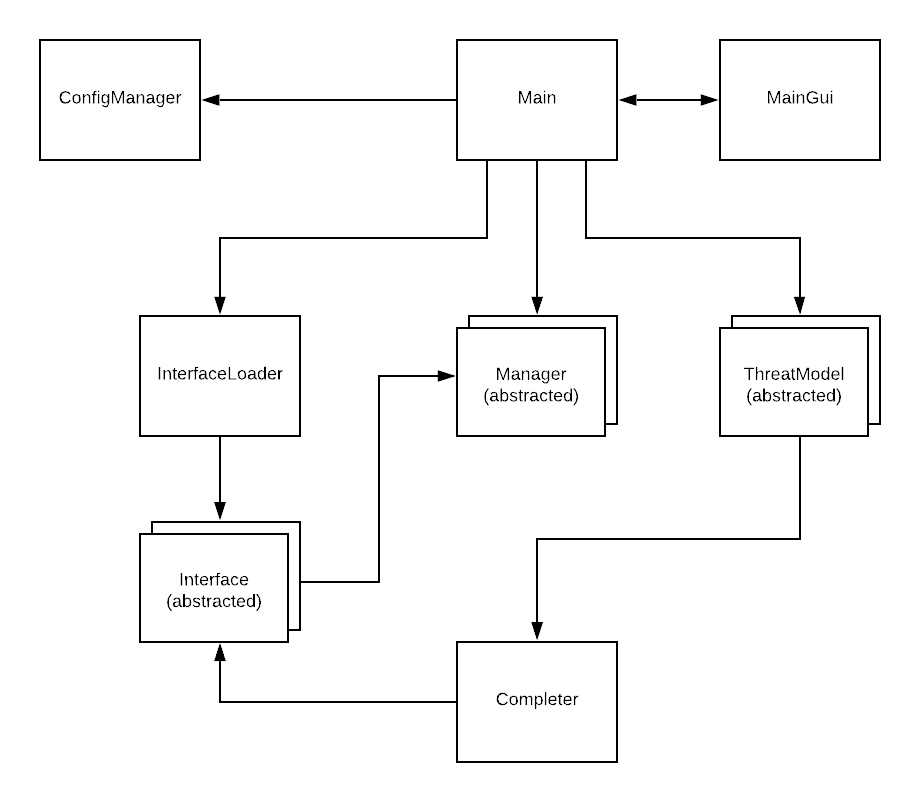
\includegraphics[width=\linewidth]
		{high_level}}
	\caption{\label{fig:high-level-struct} High level project structure}
\end{figure}

It consists of two larger and four smaller parts. The "Main" and "MainGui" components represent application parent classes. They are responsible for configuration, initialization and start up. During startup phase "ConfigManager" is called to load global system configurations such as interface folder location and cache configuration. The "Interface Loader" object is one of the central parts of the application. Its purpose, as the name suggests, is to parse penetration tool configuration files and create tool "Interface" instances. "Manager" object supervises penetration tool execution and presents output.
"Threat Model" object hides internal threat model complexity and governs its display. "Completer" object is used to link threat model data with different penetration tools and their options. It generates input suggestions during pen testing sessions. 
"MainGui" object loads the main parts of the GUI structure and controls threat model display.

Project layout diagram is provided in appendix \ref{sec:appendix-proj-struct}.


\subsubsection{Penetration tool interface}
Simplified penetration tool interface structure is presented in figure \ref {fig:interface-class} below. \newline

\begin{figure}[!htb]
	\center{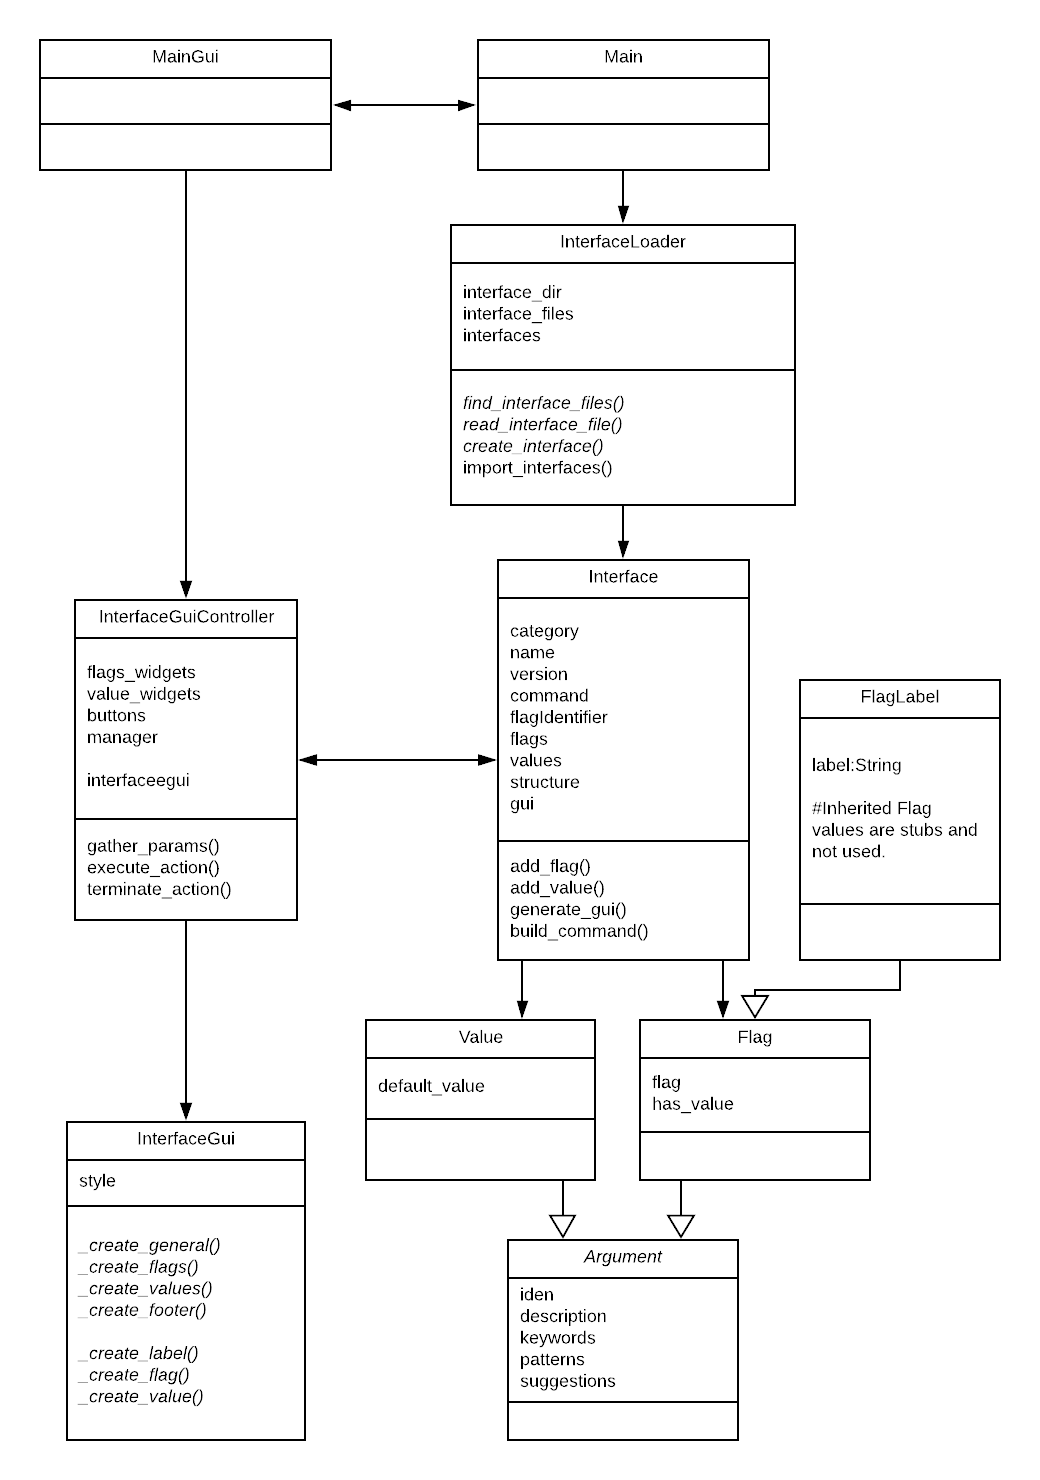
\includegraphics[width=0.8\linewidth]
		{interface}}
	\caption{\label{fig:interface-class} Simplified penetration tool interface related project part}
\end{figure}

"Interface Loader" object is responsible for finding, parsing and storing added pen testing tool interfaces. Individual penetration tools are described using their configuration files; file structure example can be found in appendix \ref{sec:appendix-config-struct}. Configuration files define tool functionality and the way to map command line options to GUI entities. "Interface" objects are individual penetration tool representations in this project. "Interface" instances encapsulate overall penetration tool information required for its use. Pen tool arguments are represented by the "Flag" and "Value" instances which are held in the "Instance" object. "Flag Label" class is used to group "Flag" instances and as a visual marker in the GUI. 

Configuration parser design is recursive; thus, "Interface Loader" only checks the general configuration file structure. Similarly, "Interface" upon receiving data is only responsible for its attributes, tool arguments are parsed by "Flag", "Value", "Flag Label" and "Argument" classes accordingly. Distributed parsing reduces complexity and splits up responsibilities making verification and testing easier.

Interface GUI is structured following MVC pattern and is automatically generated from parsed attributes. This design supports nested tool parameters without any additional configuration. However, out of projects scope, Qt library provides a markup language similar to CSS. Therefore, due to the recursive nature of the GUI design, only insignificant modifications would be needed to provide a neater user interface.


\subsubsection{Tool execution and output}\label{tool-execution}
Simplified penetration tool execution and output display diagram is presented in figure \ref{fig:manager-struct} below.
\begin{figure}[!htb]
	\center{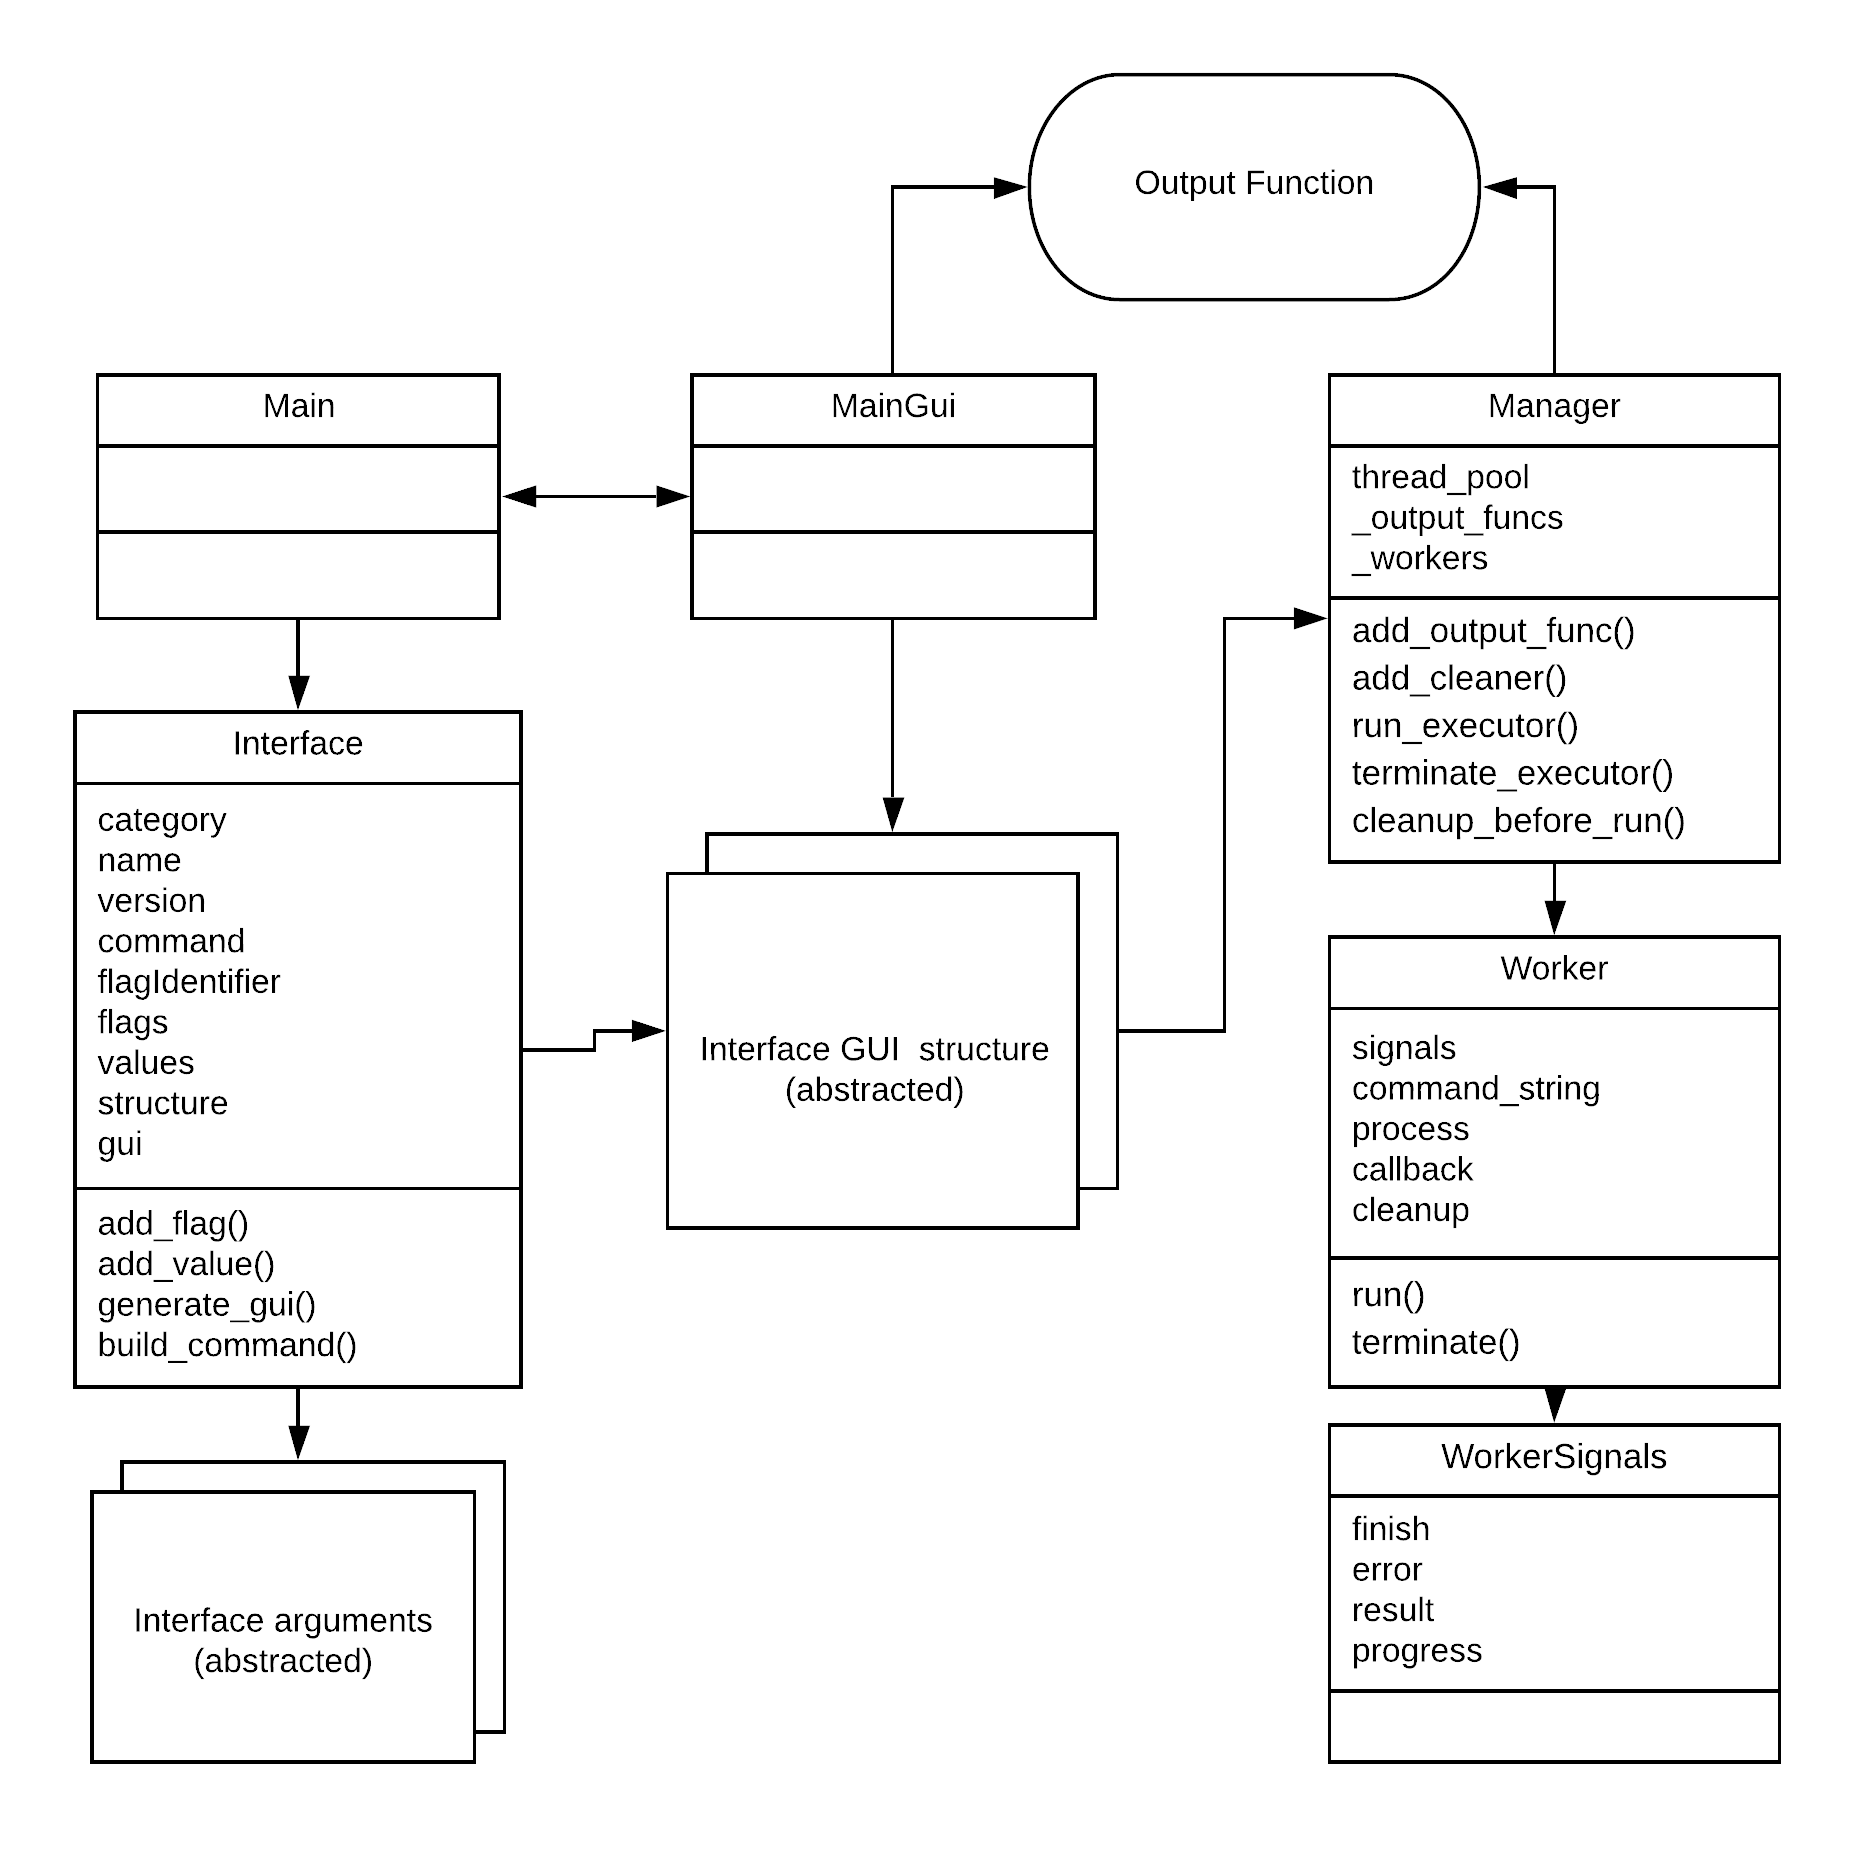
\includegraphics[width=1.2\textwidth]
		{manager}}
	\caption{\label{fig:manager-struct} Penetration tool execution}
\end{figure}

Individual pen tool (from now referred to as 'interface') execution is handled by the "Manager" object. Every interface GUI has a reference to the global "Manager" object. Upon every new interface GUI addition, a "MainGui" passes an "Output function" to the "Manager". The "Output functions" are mapped to individual interfaces inside the "Manager" object, after the interface execution they are called to display the results. Due to the variety of tools available and their visual output differences, the display functionality has been abstracted out from the system. Therefore, it is no complicated to extend the prototype with other ways of displaying the output. 

The "Manager" upon being given a command line string to create a "Worker" instance which is responsible for its execution. "Workers" start a new subprocess to run the command in the terminal. They can also receive updates on the process execution using "WorkerSignals". "Manager" can be asked to terminate a command execution which by itself will send the termination signal to an appropriate "Worker" object. When a "Worker" finishes the assigned task, it will use the "callback" function to notify the caller interface about task completion.

\subsubsection{Threat model representation}
Simplified proposed threat model implementation diagram is displayed in figure \ref{fig:threat-model-struct} below.\newline
IoT threat model described in "IoT Penetration Cookbook"\cite{cookbook} is implemented in the application threat model section. The implementation uses MVC pattern and follows Single responsibility principle\cite{single-resp}. 

The threat model internal relations are abstracted using the "ThreatModel" object. As covered in the \ref{iot-threat-modelling} section, every IoT system is composed of "Assets", which are physical or virtual entities of the system. Every "Asset" can employ a number of technologies, in this design it would be more appropriate to say that unique "Technologies" can be "used by" multiple "Assets". Every system contains multiple interaction points, here referred to as system "EntryPoints". Each "EntryPoint" is present in an "Asset". Potential system vulnerabilities are represented by the "Threat" objects. Each "Threat" is linked to a system "EntryPoint" and possible by exploiting some "Technologies" weaknesses. The individual "Threats" are then ranked using a ranking system - in this case DREAD, represented by the "DreadScore" object.

View and Controller parts are divided into multiple segments responsible only for the specific bit of GUI functionality. Threat model elements are organized using a tab menu where each tab content is generated by a different View object. Information displayed in the separate tabs is interconnected, therefore, the observer pattern is used to keep it up to date. To make user interaction more convenient, the application remembers previously entered items making the GUI more user-friendly. The item 'caching' takes place on system level, therefore, items from one threat model can be easily imported to another. Threat model front-end and back-end parts are connected view of the parent "ThreatModelController" and ThreatModel" objects.

\begin{center}
	\begin{sideways}%[htbp]
		\begin{minipage}{\textheight}
			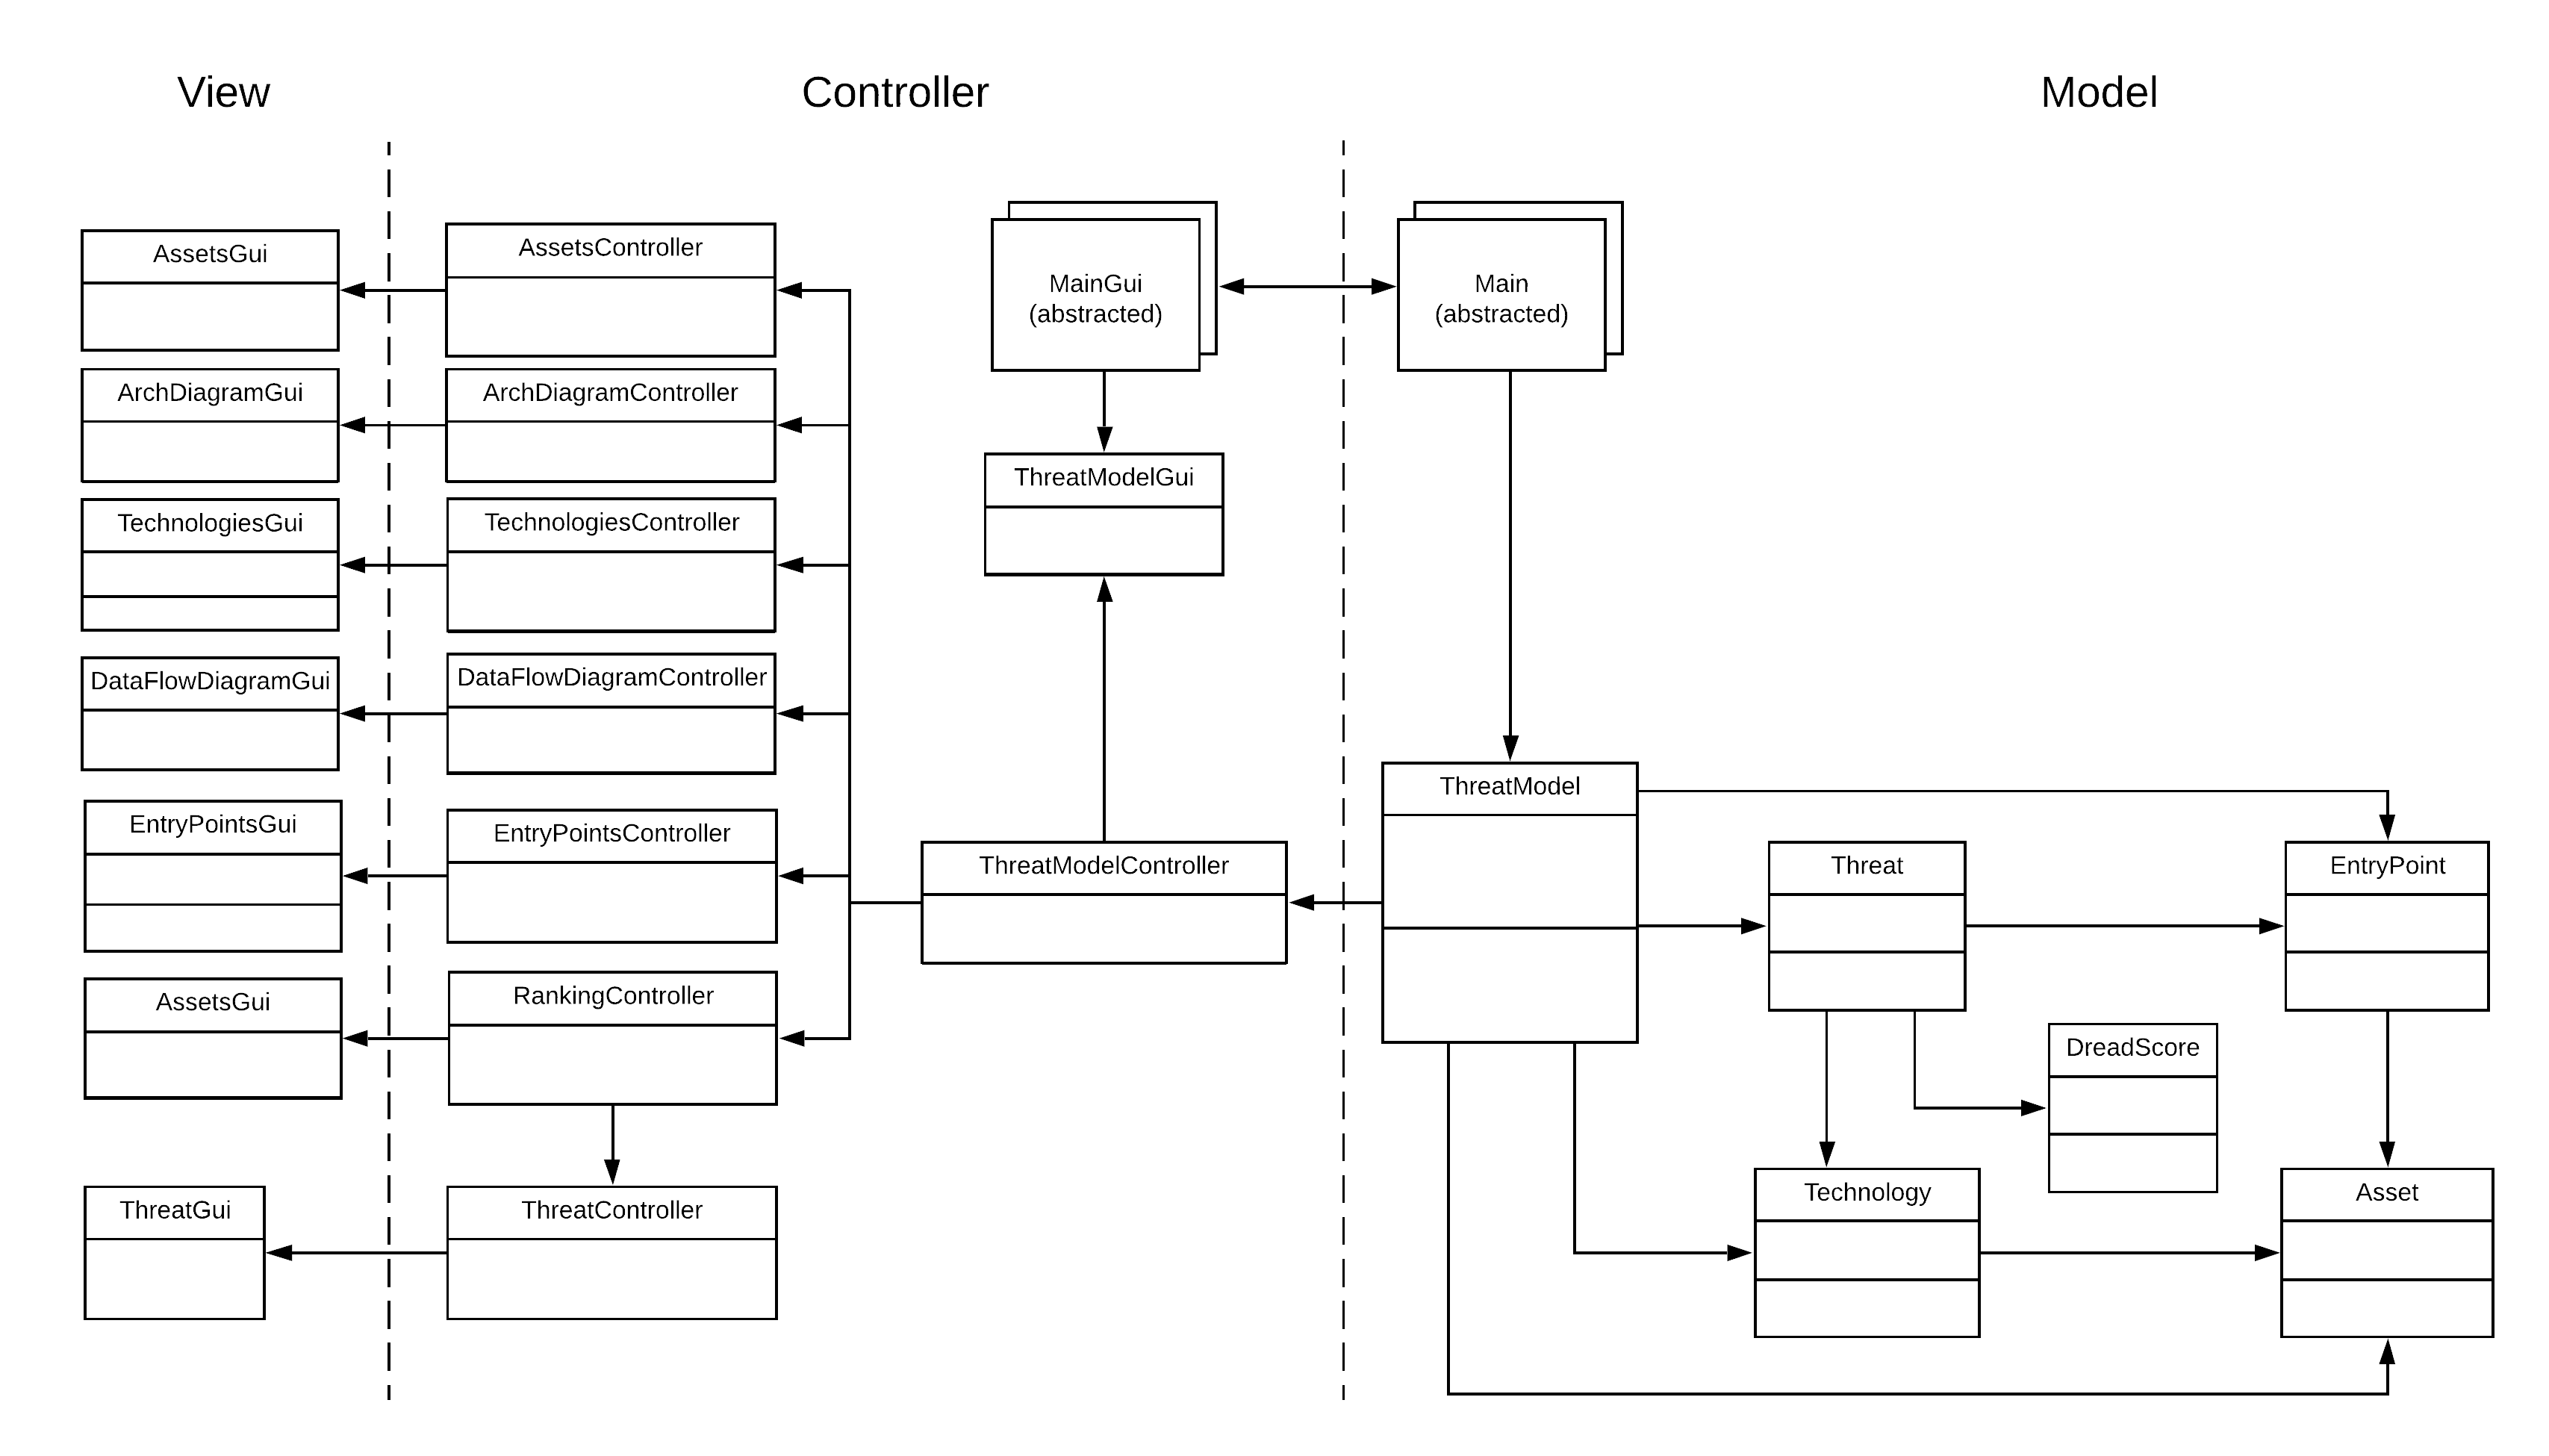
\includegraphics[width=\textwidth,keepaspectratio]{threat_model}
			\captionof{figure}{Threat Model structure}
			\label{fig:threat-model-struct}
		\end{minipage}
	\end{sideways}
\end{center}

\subsubsection{Suggestion generation}
Pen tool argument suggestion process diagram is presented in figure \ref{fig:completer} below.\newline
"Completer" object scans threat model data for specific words and phrases that match interface argument patterns. This functionality is provided as a convenience mechanism for the user linking threat model data with penetration tools included in the tool set. The "Completer" can only link keywords to assist pen tester work but at the current state cannot suggest what kind of penetration test needs to be used.

Interface configuration files can optionally contain "keywords" and "patterns" for every tool argument. These two sets of values can then be interpreted by "Completer" and matched to user entered values in the threat model. In order to separate threat information, completer requires a specific threat to be selected from the threat list. This way information unrelated to that threat is filtered out. "Completer" works by scanning every "Threat" object attribute, then the "EntryPoint" object which is linked with that "Threat" instance, then the "Asset" object of the mentioned "EntryPoint", and finally "Technologies" suspected to be used by that "Threat".

In the pen tool GUI suggestions are presented as text completion drop down list, which helps to quickly enter values for the selected test. Only tool arguments that require the user to enter information by hand may have suggestions generated; Boolean type command line arguments cannot have any values, therefore, suggestion model cannot be applied to them. 

\begin{center}
	\begin{sideways}%[htbp]
		\begin{minipage}{\textheight}
			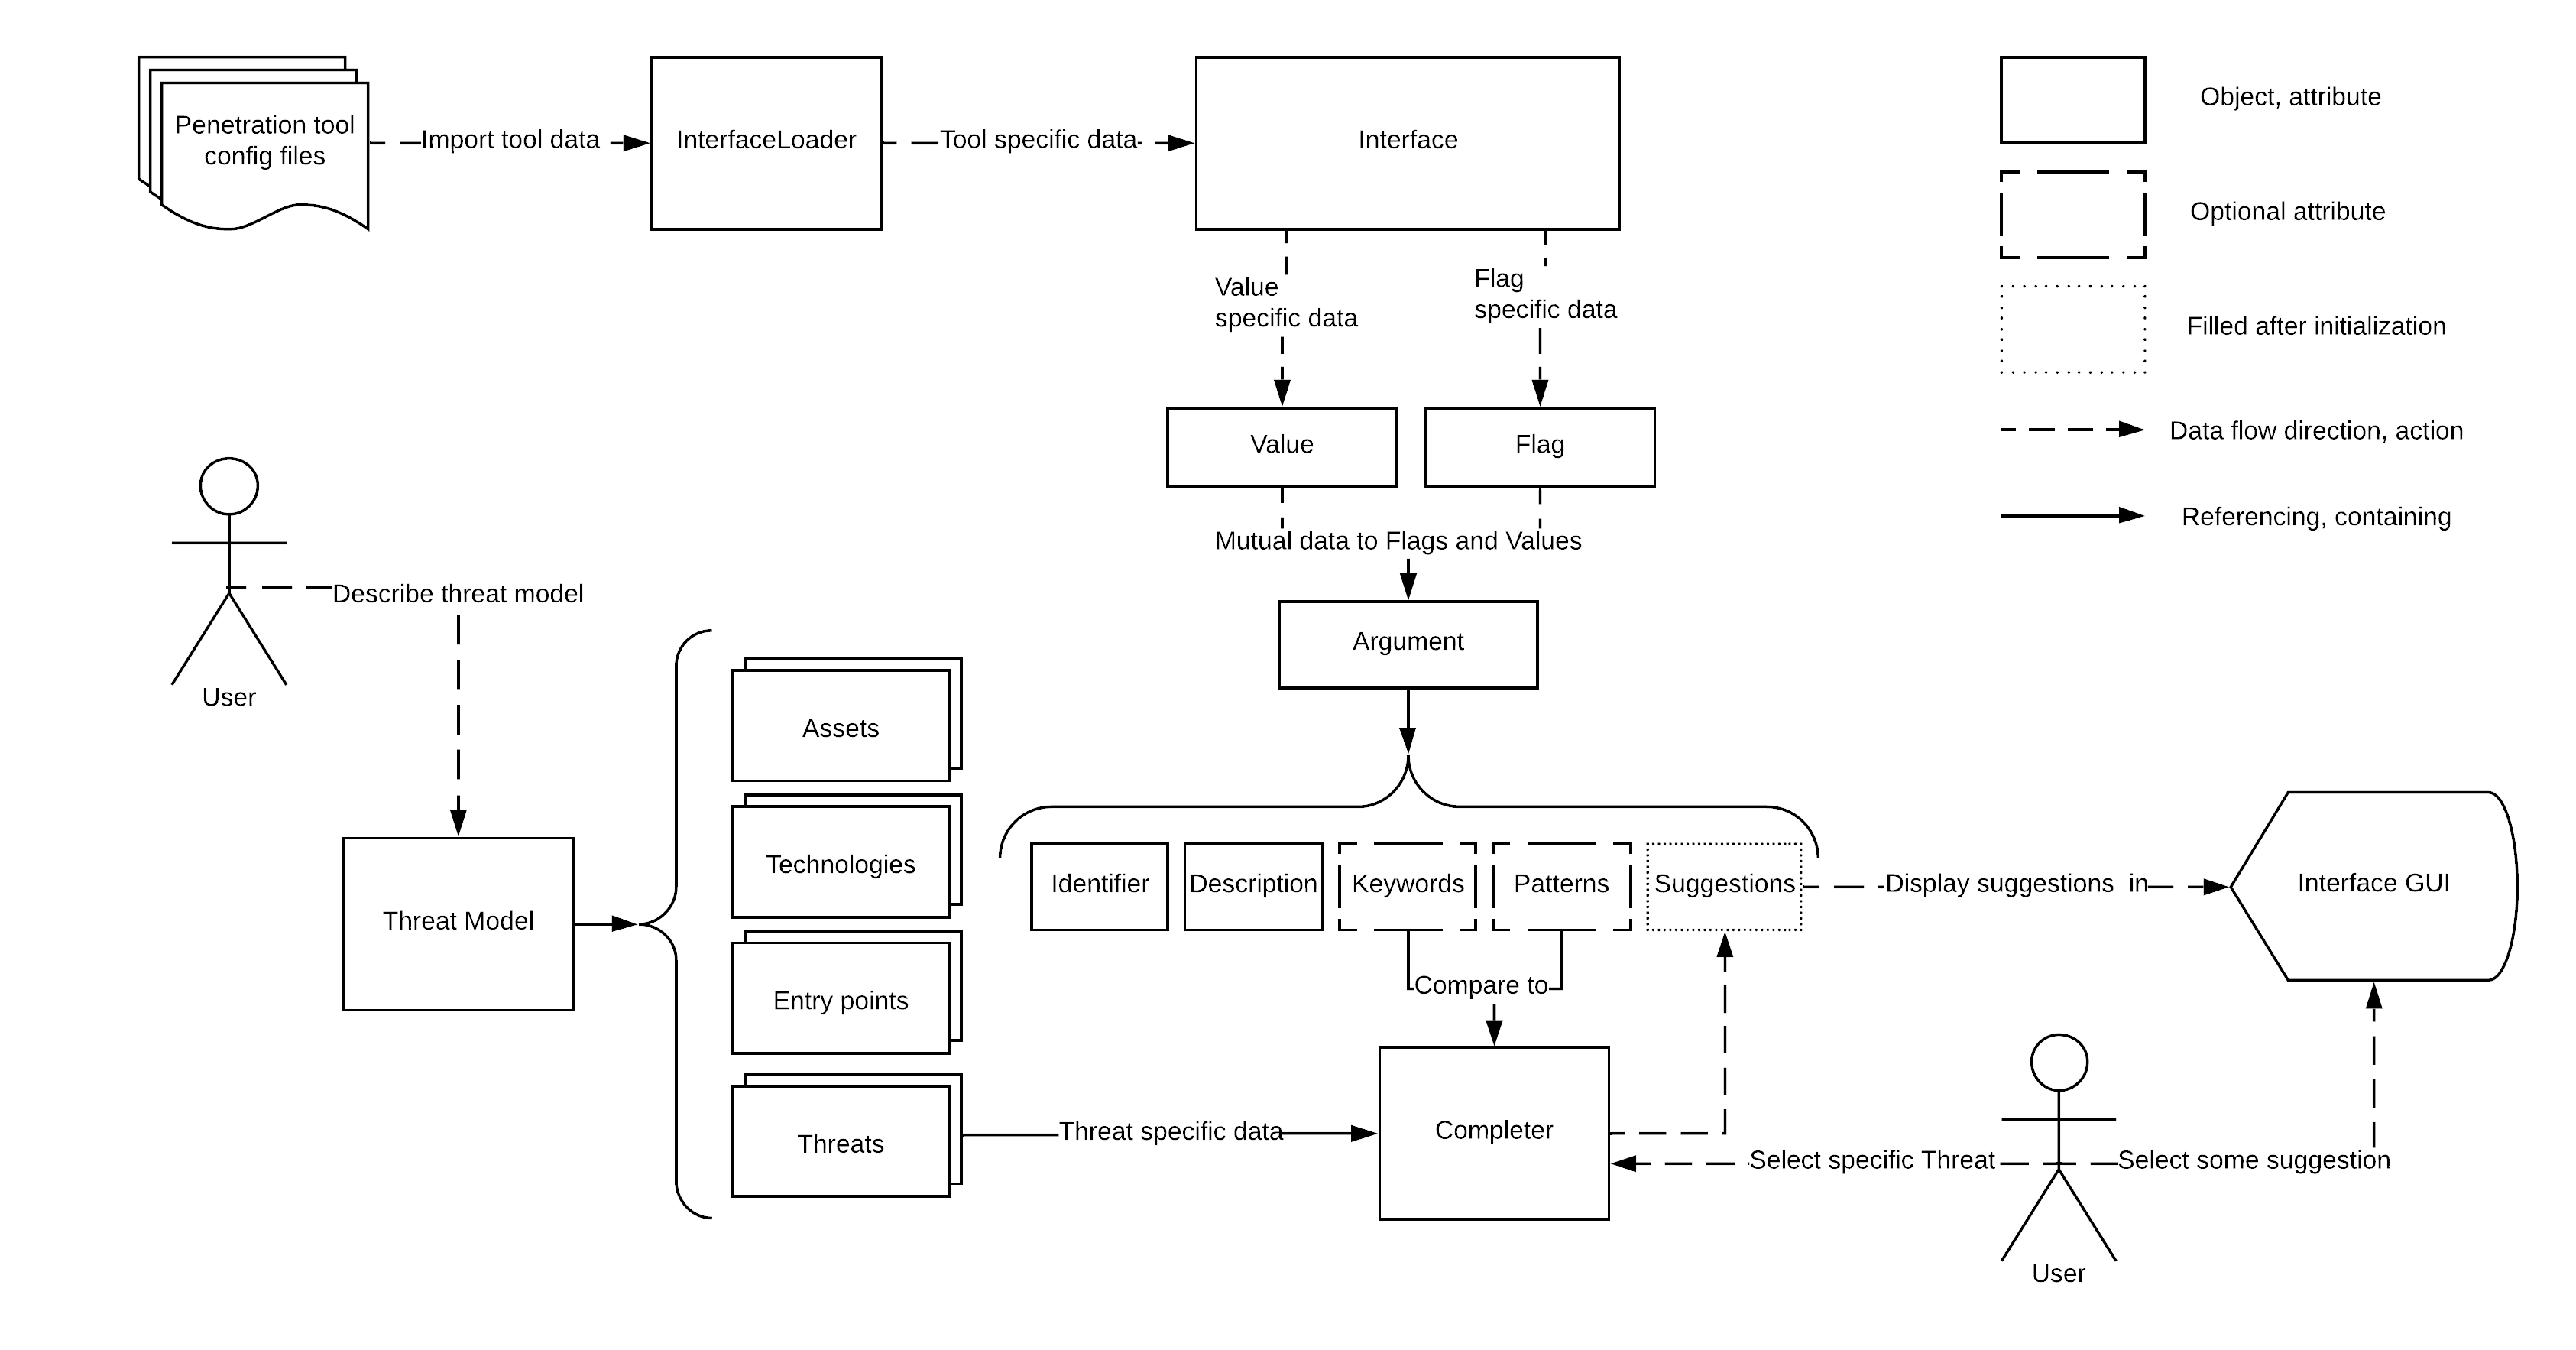
\includegraphics[width=\textwidth,keepaspectratio]{completer}
			\captionof{figure}{Suggestion generation control flow}
			\label{fig:completer}
		\end{minipage}
	\end{sideways}
\end{center}




\section{Implementation}
This section of the report covers project prototype development details more in-depth and emphasises on specific implementation decisions. It also covers the list of well-known penetration tools included in the tool set.

\subsection{Development process}
	\subsubsection{Development}
	Project prototype development has been scheduled as a continuous process during the last months of the project allowing a lot of freedom for alterations. It has been decided to follow Agile development methodology dividing tasks into Sprints and using supervisor meetings to present that Sprints results. An in depth, project management discussion is covered in section \ref{project-man}.
	
	Test-driven development (TDD) practises have been used in order to complete large amounts of robust code in limited Sprint time periods.  TDD has been used for development of the whole project back-end functionality and to test Interface GUI generation, for the front-end part has been tested using conventional testing techniques. Testing process is described in detail in section \ref{testing}.
	
	Greatest effort has been taken to follow Python PEP8 coding conventions to achieve maintainable, structured and standardised codebase. Pylint and autoDocstring VS Code extensions have been particularly useful for this goal.
	
	\subsubsection{Debugging}
	In the case of unexpected program behaviour, VS Code built in debugger has proven to be particularly useful. It's stepping through the code and break point features have been used extensively during the development process. Built in Debug console have also proven to be convenient in order to verify program objects' states and the case of exceptions or break points. 
	
	\subsubsection{Deployment options}
	After the implementation is finished, the prototype can be deployed as a Python package using dependencies management system as PIP. Installation of project dependencies would be taken care of by PIP. In order for the prototype to use tools included in it's tool set, individual pen tools would need to be installed independently in the system. Bundled program installation is one of the future work features discussed in the section \ref{future-work}


\subsection{Tool included in the tool set}
	There nine tools included in the tool set prototype. These tools have been chosen according to five areas of IoT Penetration testing\cite{cookbook}. The tool set, as mentioned before, is not by far complete but demonstrates that the prototype supports a wide range of pen tools. 
	
	Tools are grouped in sections according to their use. Only Hardware hacking section is not covered by this tool set as even if there are software tools used for Hardware related hacking, it is likely to be architecture specific and require additional physical devices or modules. Remote access section is also present in the set as it's tools functionality is rather distinct compared to other Web application or Wireless sections tools.
	
	\begin{itemize}
		
		\item Firmware
		\begin{enumerate}
			\item \textbf{binwalk} - is a tool for automated firmware extraction from the device binary image. It provides a wide range of configurations and supports different image formats.
		\end{enumerate}
	
	
		\item Web applicaiton
		\begin{enumerate}[resume]
			\item \textbf{sqlmap} - is an SQL database penetration tool. It has a powerful search engine and a range of switches configuring it's execution. The tool is useful if an IoT system is suspected to store data in a database.
			\item \textbf{wfuzz} - is a web applications brute forcing tool. It can fuzz GET and POST request parameters as well as not linked web resources.
			\item \textbf{dirb} - is a web content scanner software. It is similar to wfuzz but it uses fuzzing to discover hidden web resources and left-over files. 
		\end{enumerate}
		
		\item Mobile application
		\begin{enumerate}[resume]
			\item \textbf{apktool} - a tool for reverse engineer closed-source Android apps. It is capable of rebuilding original file structure and decode some of the initial application resources. It is intended to be used for Java based mobile applications.
		\end{enumerate}
		
		\item Remote access
		\begin{enumerate}[resume]
			\item \textbf{hydra} - hydra is a multi-process login cracker. Hydra supports a wide range of communication protocols and can be customized to try a several different approaches during it's execution.
		\end{enumerate}
		
		\item Wireless
		\begin{enumerate}[resume]
			\item \textbf{hcitool} - is a tool for configuring Bluetooth connections. It supports Bluetooth device discovery, most popular Bluetooth communication protocols and can be used to send specific commands to the Bluetooth device in order to pen test the communication.
			\item \textbf{nmap} - is the most famous network discovery and port scanner currently in the market. It is highly configurable to the point there the whole networks infrastructure can be mapped and tested by just using nmap.
			\item \textbf{sdptool} - is a Bluetooth service discovery tool. It can connect to individual discovered Bluetooth devices and retrieve information about it's advertised services.
		\end{enumerate}
	
	\end{itemize}
		

\subsection{Third-party code used}
	Apart from the libraries, which are listed in section \ref{libraries}, third party code has been used in few insignificant places in the code base:
	\begin{itemize}
		\item In the file \textit{line.py} for custom Qt GUI element implementation.
		\item In the file \textit{vtabwidget.py} for rotating the Qt GUI tab container titles.
		\item In the file \textit{manager.py} for implementing \textit{WorkerSignals} communication model.
	\end{itemize}
	In all of the occurrences, appropriate headers have been used to clearly indicate third-party code.

\subsection{Implementation details}
	This subsection covers some important implementation details that were not covered in the Design section.

	\subsubsection{Application preferences file}
	The program has a global preferences file which is used to define application level settings. Following Python conventions, such information is stored in a '.ini' file, which is then parsed and maintained with built-in Python "configparser" library. In the case of complete loss of the configuration file or one of it's mandatory fields, a new '.ini' file is populated using reasonable default values.
			
	
	\subsubsection{Interface file structure}
	Penetration tools used in the tool set are referenced via their "interface\_x.yaml" files. Each file has mandatory and optional fields. An example interface file is shown in appendix \ref{sec:appendix-interface-struct}.
	
	The file is in YAML format which was chosen due to it's simplicity, readability and compatibility. As these interface files have to be configured by hand for every penetration testing tool, intuitive structure and readability was a priority. If for example, XML format was chosen, it would be much more complicated for the human to compose configuration files.
	
	It is important to note that tool flag and value lists can be empty and can be defined recursively (e.g. flag containing optional flags). Configurations described in YAML format are easily appendable and auxiliary fields would just be ignored.
	Adding a new tool to the system is as simple as creating a new interface file from the example and adding it to the appropriate folder.
	
	
	\subsubsection{Graphical User Interface functionality}
	Care has been taken to make the application GUI intuitive and simple to use. 
	The application takes extensive use of tabular structures. Penetration tools are grouped according to their purpose using separate tabs. Threat modelling project part uses two levels tabular structure to group related functionality. 
	Every threat model entry can be edited, duplicated and deleted. 
	Threat model items (e.g. entry points) are cached on the application level, thus can be reused in other projects, cache can easily be cleared for separate threat model item groups (e.g. technologies).
	Threat models can be loaded, edited and saved again, appropriate warning messages are thrown while trying to close threat model with unsaved information. Threat models can then be exported as json files for data visualization. Appropriate native hotkeys can also be used for these operations. 
	
	
	\subsubsection{Scalability}
	Prototypes scalability is twofold. On one hand, the application can easily import as many tool interfaces as provided and load threat model files as big as needed. On the other hand, large files were not taken into consideration during the development process and no special action have been taken to parallelize or divide any of the tasks in any way. Effort has been made to use native GUI element as scrollbars to display large information sections and separate GUI functionality using tabs. Nevertheless, it may be inconvenient for the use to navigate through large numbers of tools and threat model items.
	
	As described in section \ref{tool-execution}, penetration tool execution and output generation is parallelized using functional programming, therefore, tool execution scalability is only dependant on users hardware.
	


\section{Testing}

\subsection{Software testing}

	\subsubsection{Unit testing}


	\subsubsection{Integration testing} % for interface gui generation


	\subsubsection{Usability testing}


\section{Project management}
\section{Evaluation}
	
	\subsection{Requirements evaluation}
	The prototype provided complies with all but one previously defined functional and all but one non-functional requirement. 
	
	Importing or removing penetration tools from the tool set is uncomplicated by moving interface files from the dedicated folder. The proof-of-concept tool set contains various tools including the ones for LAN network scanning and Bluetooth communication protocols. The implemented threat model is designed to be updated with new data from the penetration test runs, as well as mapping appropriate keywords from the threat model to the individual penetration tools. After testing is completed, the threat model together with the included testing results can be exported as structured; JSON output to be used later or displayed in a separate report. 
	The functional requirement which was not met is the tool output chaining. This specification had to be refused due to its complicated nature involving universally supporting parsing of penetration tools output and its limited cases of use.
	
	The tool has been tested and run on Ubuntu OS using Python and Pip package manager which guarantees its compatibility with other Linux operating systems that support the required dependencies. It also implements multithreading, thus, moving all the computationally intense tasks away from the main program threat and ensuring quick program response. The prototype does not scan for devices on the network itself but employs well-known pen tools to complete these tasks, it shifts the responsibility to Nmap and Hcitool implementations which can perform scans on huge networks without any difficulties. 
	The unfulfilled, non-functional requirement was the complete encapsulation of the tool in one portable program. Due to a shorter development period and the relatively low additional value of this feature, the requirement was not completed. The prototype packaging is somewhat finished as third-party dependencies can be installed automatically using a package manager.
	
	The final result is in accordance to the project Brief included in Appendix \ref{sec:appendix-preject-brief} and the project goals raised at the start of development process are met. A slight shift from the project brief goals is that the final prototype focuses on the use of IoT penetration methodology and not just penetration testing.
	
	\subsection{Usability and testing}
	The tool usability has been evaluated during an actual IoT alert system penetration testing. The system was tested using "grey box" method which combines internal system knowledge with the outside attacker methods. The IoT penetration tool proved to be usable and suitable for this kind of penetration testing, nevertheless, additional work in tools GUI design would be welcomed.
	
	The tool has been tested with a combination of unit and integration tests with an emphasis on the tools back-end functionality. The front-end and GUI testing has been done manually and by doing the evaluation of the alert systems.
	
	\subsection{Future work}\label{future-work}
	A few parts of the IoT penetration tool could be improved in the future. \newline
	At the current moment, the system can pipe penetration tools output to any destination, however, only the most basic terminal-like display is included. A more user-friendly way of presenting penetration tools output would greatly improve the usability of the tool. During the project development it was decided to implement a generic approach as individual penetration tools use their own output formatting and may support other forms of data representation. As the tool is aimed at supporting any command-line based penetration tool, a generic approach which can be extended to other formats, makes more sense. 
	
	For the prototype to include advanced tool functionality GUI design has been neglected and a properly formatted GUI could make the tool more readable. As the tool GUI design is not optimized some options or fields are not displayed in the most efficient manner. The same could be said for the colour scheme and text font styles.
	
	Effort could potentially be made to expand the current tool set by writing interfaces for a package sniffer or for penetration tools used in other areas e.g. firmware analysis. As the project requirement was to provide an extendable penetration tool platform and a proof-of-concept tool set, only the basic cases of use are covered. 
	
	Some additional work could also be done for the tool to convert structured threat model format into a user-friendly interactive report displaying key penetration testing results. The prototype provides structured data which could be represented in any way and in any format needed. Report generation in a particular form would limit the gathered information to a single format that could not be easily reused. 
	
	\subsection{Conclusion}
	This project addresses the rise of IoT related cyber security risks and their exploitation. It provides a platform where threat modelling is combined with penetration tools. The tool is trying to fill the void of dedicated IoT penetration testing solutions which could be used by people with little cyber security related experience. It is essentially a highly extendable IoT penetration testing platform closely linked with IoT threat modelling methodology. The two are coupled in order to guide the user to properly structure and document the penetration testing process. The proposed "IoT Penetration Testing Toolset" could also be called a penetration testing assistant as it helps the user to structure the system evaluation process. It is hoped that the tool would assist in creation of more secure consumer and industry level IoT systems.


% \section{Introduction}

Modern society seamlessly adapted to using gadgets and appliances that 30 year ago only existed in futuristic science fiction movies. Smart devices have slowly become part of everyday lives. Self driving trucks are not something out of a distant future anymore\cite{freedman_2017} and Internet connected appliances such as light bulbs and  smart coffee makers are finding their places in common people homes. It was estimated that in 2017 there were around 27 billion connected IoT devices around the globe. This number is expected to increase by around 12 \% each year until it reaches 125 billion by 2030 \cite{ihs-markit}. For comparison in 2014 there were around 1.57 billion smart phone owners worldwide, this number is bound to reach 2.87 billion by 2020 \cite{statista}. Although, smart phone numbers are growing fast, they are limited by the number of people using them. This is not the case with smart Internet of Things devices. For example an industrial factory may contain hundreds of different sensors. The IoT networks and stand-alone "Smart things" technologies are booming \cite{gartner2018} and will only increase in numbers. Unsurprisingly, such growth is starting to cause privacy, security and regulation concerns as it is hard to control. Even though these technologies have greatly complimented people lives one can not stop wonder are their owners properly manage these numbers of Internet connected devices.

Even though IoT devices collect incredible amount of users sensitive information and it is starting to cause processing and security concerns \cite{7069995} little is being done to properly secure these devices. As it has been shown by the Mirai botnet attack in 2016, IoT technologies can be used to create record breaking botnets and disrupt more traditional Internet services\cite{203628}. If proper measures are not taken it is likely that more large scale malicious IoT network exploitation will take place. As the manufacturers are pushed by market growth to develop new products faster in order to keep up with their competitors proper security testing is becoming luxury that usually can not be afforded. Moreover, it appears that consumers are not concerned about their device security\cite{iotm}. As studies have shown even Internet connected vehicles can be hacked into and controlled remotely\cite{8071577}. As Internet connected devices are exposed to many more threats than a non-connected electronic devices steps must be taken to ensure IoT gadgets and Internet connected devices are robust and safe to use.

Due to vast differences in deployment environment as well as technologies in use proper IoT technology testing is difficult to ensure. One reason severely complicating the testing process is the use of third-party technologies and services. A single IoT device firmware may be written by a mix of contracted developers known as Original Design Manufacturers (ODM) and in-house developers hired by hardware manufacturer Original Equipment Manufacturer (OEM), then the application code itself may be supplied by a completely different company\cite{cookbook}. The problem occurs when OEM and ODM merge code bases. The ODM may provide only the binary files or an SDK for the OEM. Therefore, if that happens Original Equipment Manufacturer which is responsible for distributing firmware, managing it and releasing updates, does not have full access to the code. Moreover, IoT networks are comprised of many different kinds of devices that are responsible for different functions. Each individual device may be manufactured by different suppliers and their OEMs accordingly. As no individual link of the supply chain posses access to the full infrastructure source codes, it may be impossible to thoroughly test the system as a whole. It becomes apparent that black box type penetration testing and vulnerabilities scan may be the only acceptable strategy in order to secure complicated IoT systems.

As the field in question is rather new, diverse and rapidly developing it is complicated to find knowledgeable specialists and tools developed specifically for IoT penetration testing. There are numerous blogs and projects offering various level of detail guides to IoT penetration testing\cite{github}. Some organizations including IEEE and ETSI have released technology-specific standards as well as security guidelines but non try to cover IoT in general\cite{Zhao:2013:SIT:2584913.2585964}. 

The purpose of this project is to try to simplify IoT penetration testing. It summarizes the general concepts of IoT penetration testing and present them in a user friendly manner. Moreover, this project tries to address the lack of dedicated IoT penetration testing technologies and provides an extendable framework which purpose is to reuse existing penetration tools to test IoT systems. The tool is designed to require little technical knowledge and is highly modifiable in order to adapt to particular IoT infrastructure.

This report is divided into sections starting with an abstract and introduction. The subsequent parts of this report background research and investigates the most commonly used IoT technologies and protocols up-to-date. Afterwards, distinct goals and requirements are listed for this project. They are followed by explanation of design decisions and the general structure of the application. This report is finalized by listing remaining work and explaining project management decisions taken up to this point.

\section{Background research}
There is no clear definition of the Internet of Things technologies. Some define it as "the concept of every device blending with the existence of human beings"\cite{DBLP:journals/corr/MendezPY17}. Which basically means that there would be no difference between human and device interaction with the system. In it's simplest form IoT systems can be defined as decentralized networks there multiple, usually, limited capabilities embedded processing units communicate between each other in various ways. The fact that they have communication capabilities implies that they can change their behaviour depending on input received via network. That is what exposes "smart objects" to outside threats\cite{riahi:hal-00868362}. This increases the penetration testing complexity from a single isolated embedded device to a distinct Internet entity that requires a new layer of security. Addition of a network interface transforms a narrow purpose device into an interactive network component.

Insertion of previously isolated technologies into the global Internet network attracts malicious users attention. Unprotected log-ins, outdated software and insecure communication would not cause major security issues for hidden away, stand-alone embedded devices as long as they function properly (e.g. medical equipment). The situation is the opposite if a device can be discovered and interacted with by anyone on the network. Moreover, IoT devices can be extremely favourable targets to hackers which are expanding their bot networks. Unlike regular computers, IoT devices usually run continuously without halting and can be exploited without owners knowledge\cite{191952}. It seems that traditional approaches of securing devices are not effective\cite{DBLP:journals/corr/abs-1803-05022} due to IoT technologies uniqueness and variety.

Above listed problems require penetration testing to be taken in several layers, breaking down IoT network infrastructure and exposing separate attack vectors. Testers must take into account 6 different aspects of IoT infrastructure. Hardware vulnerabilities can be exploited by anyone who has physical access to the device. Such vulnerabilities may be an open debugging port, password reset button and tapping into hardware level communication (e.g. UART)\cite{attify}. Firmware in this context stands for device operating system which can be rather primitive or extensive and using third party SDK and libraries introducing possible vulnerabilities\cite {cookbook}. Application level vulnerabilities usually happen due to a software bug or a logic error\cite{cookbook}. Communication and network exploits happen due to man-in-the-middle attacks and usage of insecure communication protocols assuming security by obscurity. If a device or an IoT system has a web interface, it essentially becomes a web host, thus it may have all the vulnerabilities of a regular website\cite{2007:WAH:1406550}. Lastly, some IoT vendors release mobile applications complimenting their products. That is another new and troublesome attack vector as hackers may get access not only to victims IoT devices but also get a foot hold in user smart phone possibly accessing sensitive information stored in there\cite{cookbook}. Only by addressing each part of the infrastructure individually and as a whole one can truly secure IoT systems.

The most popular and the most convenient method to interact with an IoT device is via wireless network. There are many different communication technologies developed for this purpose. All of them were designed to accomplish specific tasks, therefore they vary in range, connection speed, energy consumption and security. Some of the most widely used are WiFi, Bluetooth, ZigBee, GSM and Z-Wave \cite{cookbook}. To devise a proof of concept, two different protocols are sufficient, therefore this project will concentrate on WiFi and Bluetooth communication. WiFi is based on IEEE 802.11 standards, it is no different to LAN communication. The two most ways of sending information is UDP and TCP protocols which act very differently \cite{4359944}. By itself WiFi communication is not encrypted, therefore if application developers did not secure ongoing traffic, such data is vulnerable to network sniffing attacks. Recent versions of Bluetooth, contrarily have built-in encryption, therefore sniffing it is rather complicated \cite{scarfone2012guide}. Nevertheless, Bluetooth devices are still vulnerable when they connect to an end-point for the first time (pairing) \cite{scarfone2012guide}. It is easier to exploit specific protocol vulnerabilities with tools already designed for that purpose. As the tool set is designed to take re-use best parts of already trusted penetration tools, it will be able to retain generality still succeeding in fine-grain testing.

\subsection{Threat modelling}
According to the "IoT Penetration Testing Cookbook"\cite{cookbook} threat modelling can be broken down into these steps:
\begin{enumerate}
    \item Document all system assets using publicly available information: try to identify each device, write down all applicable information that may provide any hints on systems internal processes.
    \item Create architecture overview:
    \begin{itemize}
         \item Document IoT system functionality and features, create use cases
         \item Create architectural diagram that shows what components control flow
         \item Using architectural diagram and created use cases identify each individual component and communication method system communication method.
    \end{itemize}
    \item Use acquired system picture to identify entry points and write down possible threats. It does not have to be exact but it has to be backed up by some evidence.
    \item Starting with most likely threats determine:
    \begin{itemize}
        \item Threat targets 
        \item Possible exploitation techniques
        \item Possible countermeasures
    \end{itemize}
    \item Rate threats using DREAD rating system\cite{dread} and group them accordingly (High 12-15, Medium 8-11, Low 5-7)
    \item After the overall system analysis is finished, repeat the same process examining each part of the IoT system separately. Reuse previously created mapping and include new information reflecting on device specific threats. This is the time to logically and realistically evaluate each part of the system.
    Writing down possible threats for individual devices, mapping attack surfaces and identifying vulnerabilities which may lead to exploitation of distinct device weaknesses.
    \item Final step is to analyze and attack top ranking vulnerabilities of each system component (firmware, mobile application, communication, etc.) looking for a way in.
\end{enumerate}


\section{Project Goals}
This project goal is to collect information about IoT penetration testing and provide a tool that allows the generalized methodology to be easily applied in practise. The tool should be able to execute different types of network scans and display discovered devices in a user-friendly manner. The tool is also supposed to be able to apply information gathering techniques to individual devices such as port scanning. The idea is to visually present device and network specific information gathered from automatic and manual tests to get a better understanding of the system. By following penetration testing methodology it is then possible to identify attack surfaces and exposed entry points.

With initially gathered information a user can then choose one of the modular tools added to the application and apply device or protocol specific tests. The biggest advantage of a tool like this is its ability to use preexisting penetration tools to achieve individual tasks. As the IoT technology stack is so diverse it is impossible to design a tool that covers all the use cases. Instead, this project should provides a "tool box" which comes with a few basic testing tools and ability to add new tools if a need arises. The basic tools allow users to get a first view at the system of interest and make decisions about the next step.

As one of the emphasis of this application is to make IoT penetration testing more accessible and coherent for a diverse audience the ease-of-use and simplistic design are key aspects of the application. The whole tools functionality needs to be accessible via a graphical user interface with hints and explanations reducing the learning curve.

\subsection{Requirements}
    \subsubsection{Functional}
        \begin{itemize}
            \item Functionality to add and remove new security tools to and from the application
            \item Contain an initial proof-of-concept set of tools
            \item Scan local network, map network infrastructure and identify its components
            \item Support at least 2 communication protocols: WiFi and Bluetooth
            \item Provide guidelines and best practice for IoT penetration testing
            \item Give suggestions of most likely vulnerabilities in response to the initial network scan
            \item Allow chaining separate tool execution
            \item User is able to interact with the application via a graphical user interface
        \end{itemize}
    
    \subsubsection{Non-functional}
        \begin{itemize}
            \item Contains all required dependencies and is portable with little to no setup
            \item Compatible with most popular Linux distributions
            \item Must provide user with feedback within 2 second of user interaction
            \item Must be able to identify at least 25 unique devices on the network
        \end{itemize}

\subsection{Limitations}
This project cannot possibly find all existing IoT device vulnerabilities nor address specific firmware or hardware details; thus, it will only check for most frequent IoT device weak points. The tool set concentrates on finding application and communication level vulnerabilities. Some communication protocols may require special hardware tools and are harder to test. Because of the modular nature of the application design it may be possible to use such tools e.g. for capturing GSM communication packages \cite{DBLP:journals/corr/ShaikBANS15} but due to time and resource limitations it is out of scope of this module. It is also impossible to use the same technique to test an area as diverse as IoT networks. Therefore, the methodology provided is only guidelines gathered from multiple sources and may need alterations.

\subsection{Risk analysis}
Probability and Impact are rated in a scale from 1 to 5.

\def\riska{Loss of source code at some stage of development}
\def \probabilitya {1}
\def \impacta {4}
\def \mitigationa {Use of remote source control  repository to frequently record every stage of the development, thus being able to recover it if needed. }

\def\riskaa{Unable to fulfill all of the requirements due to technical implemention difficulties}
\def \probabilityaa {3}
\def \impactaa {2}
\def \mitigationaa {During the start of development process requirements will be split into tasks, divided into sprints and ranked using Agile methodology, therefore ensuring that core functionality will be implemented first and a working proof of concept is available at the end of the project }

\def\riskaaa{Loss of development time due to other course modules}
\def \probabilityaaa {2}
\def \impactaaa {2}
\def \mitigationaaa {Dedicate fixed amount of time every week for the project in order to keep up with the schedule }

\def\riskaaaa{Some part of the project taking up significantly longer that expected}
\def \probabilityaaaa {3}
\def \impactaaaa {2}
\def \mitigationaaaa {Re-evaluate task importance and readjust development schedule in order to deliver functional prototype }

\def\riskaaaaa{Unable to complete adequate application testing due to technical or time limitations}
\def \probabilityaaaaa {3}
\def \impactaaaaa {3}
\def \mitigationaaaaa {Complete limited or partial testing concentrating on core functionality, document causes and reasoning. If difficulties arise in early stages of development  due to technical limitations, seek support from university staff that have more experience in similar situations. }

\begin{center}
\begin{tabular}{ |m{5cm}|m{2cm}|m{1cm}|m{6cm}| } 
 \hline
 Risk & Probably & Impact & Mitigation \\ 
 \hline
 \riska & \probabilitya & \impacta & \mitigationa \\ 
 \hline
 \riskaa & \probabilityaa & \impactaa & \mitigationaa \\ 
 \hline
 \riskaaa & \probabilityaaa & \impactaaa & \mitigationaaa \\ 
 \hline
 \riskaaaa & \probabilityaaaa & \impactaaaa & \mitigationaaaa \\ 
 \hline
 \riskaaaaa & \probabilityaaaaa & \impactaaaaa & \mitigationaaaaa \\ 
 \hline
\end{tabular}
\end{center}



\section{Application design}
The penetration testing tool is chosen to be a desktop based GUI application. Desktop applications will have no dependencies on browsers. Server side - client side code complications and JavaScript engine dependencies are also removed. It is planned that all libraries and resources required for the application to run would be included in the final deliverable, thus increasing portability and reducing setup complexity. Additional features as automatic update service and application error scan is planned in order to keep software up to date by using git repository as a code base.

Application will implement modular design to re-use existing penetration tools and follow usage-centered design principles. In order to add a tool to the tool set, a user will have to define an interface/wrapper for the new tool. The wrapper will contain instructions on how to convert GUI input to tool specific commands as well as interpret tools output. This design allows flexibility and makes no assumptions about individual tool input or output. By prioritizing usability and clarity the application will remain user friendly and minimize new users learning curve \cite{user}.

It has been decided that the application will be written in Python. Python is a dynamic scripting language suitable for rapid development and prototyping. There will be no learning curve to use it as work experience is already present. Graphic User Interface will be developed using PyQT library as it is highly customize and popular between Python developers. Python is also by default present in the majority of Linux distributions, therefore no additional setup will be required. Other alternatives as Java, JavaScript and C++ were considered but were dismissed due slower development cycle, steeper learning curve or lack. One may point out Python lesser performance as a disadvantage but as the majority of computationally heavy tasks will be executed by other tools that does not make any difference.

A UML diagram present describes general application structure.

\begin{figure}[h!]
\caption{UML diagram}
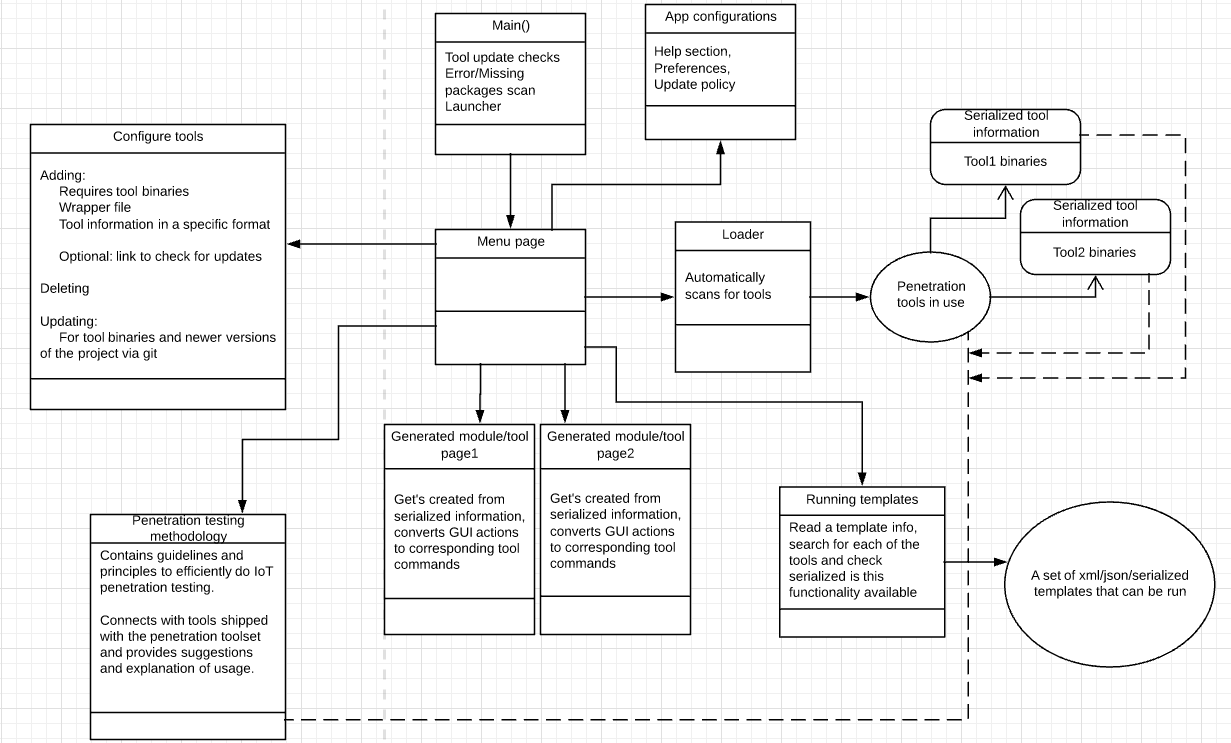
\includegraphics[width=\linewidth]{UML-diagram}
\centering
\end{figure}

\section{Remaining work}

Work completed up to this point and the remaining work is visualized using Gannt chart. The application design and background research phases are completed. The remaining development time will be mostly divided into sprints of 10-14 days in order to assign time for inevitable other module assignments. Each sprint will have a predefined set of tasks prioritized in Agile manner. After the sprint is completed planned functionality is supposed to be fully functional and tested to constantly add value. The Christmas period, January exam period and Easter periods are planned in looser manner in order to accommodate vacations, assess progress and re-think design decisions. The last weeks of the project are reserved for writing final report.

\begin{figure}
\caption{Gannt chart}
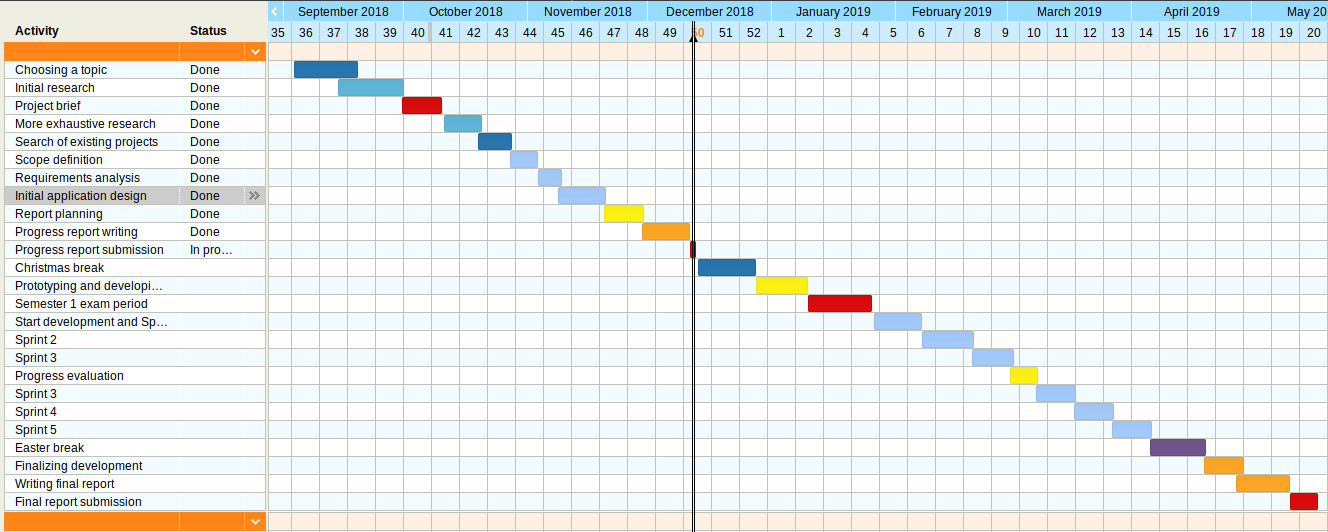
\includegraphics[width=\linewidth]{Gannt}
\centering
\end{figure}
\newpage
\bibliography{references}

\section{Appendices}
\appendix


\section{Project brief}\label{sec:appendix-preject-brief}

Internet of Things (IoT) Penetration Testing Toolset

Sarunas Iljeitis (si1g16)

Supervised by Dr Julian Rathke (jr2)

\begin{enumerate}
	\item Problem:
	
	Nowadays people tend to use more and more low-end consumer-based electronics. Such sensor based or smart-devices are used to create highly automated networks (IoT networks) that assist humans in performing various tasks. Unfortunately, product manufacturers are driven by ever-increasing demand for highly functional affordable gadgets, because of that security is usually not their top priority. The current IoT gadget market is filled with low-quality inexpensive devices that implement poor security standards. Some security vulnerabilities could be easily prevented by device users simply following mutual security standards guidelines. As consumers are usually negligent to properly secure their new gadgets and device manufacturers are more concerned about minimizing the production cost such devices become favorable targets for attackers wishing to compromise owner’s network.
	\item Goal:
	
	Penetration testing is an essential aspect of any modern device, application or network development. It is the single most effective way of finding security breaches before the actual attack happens. The goal of this project is to provide a set of tools that can be automatically applied to IoT networks or individual devices to scan for common IoT vulnerabilities. The toolset is intended to be used to find vulnerable devices which use different communication methods, apply customizable vulnerability tests and provide test results in a report. The toolset would follow most common IoT device testing methodology and vulnerability testing best practice.
	\item Scope:
	
	This project cannot possibly find all existing IoT device vulnerabilities nor address specific device level implementation details; thus, it will only check for most frequent IoT device weak points. The toolset will concentrate on testing mutual device properties providing a certain level of configuration for different tests following common testing patterns. It will not however be able to expand over bigger IoT infrastructures as it concentrates on testing singular devices or a small set of devices on the same network.
\end{enumerate}


\section{Class diagram}\label{sec:appendix-class-diag}

\begin{center}
	\begin{sideways}%[htbp]
		\begin{minipage}{0.92\textheight}
			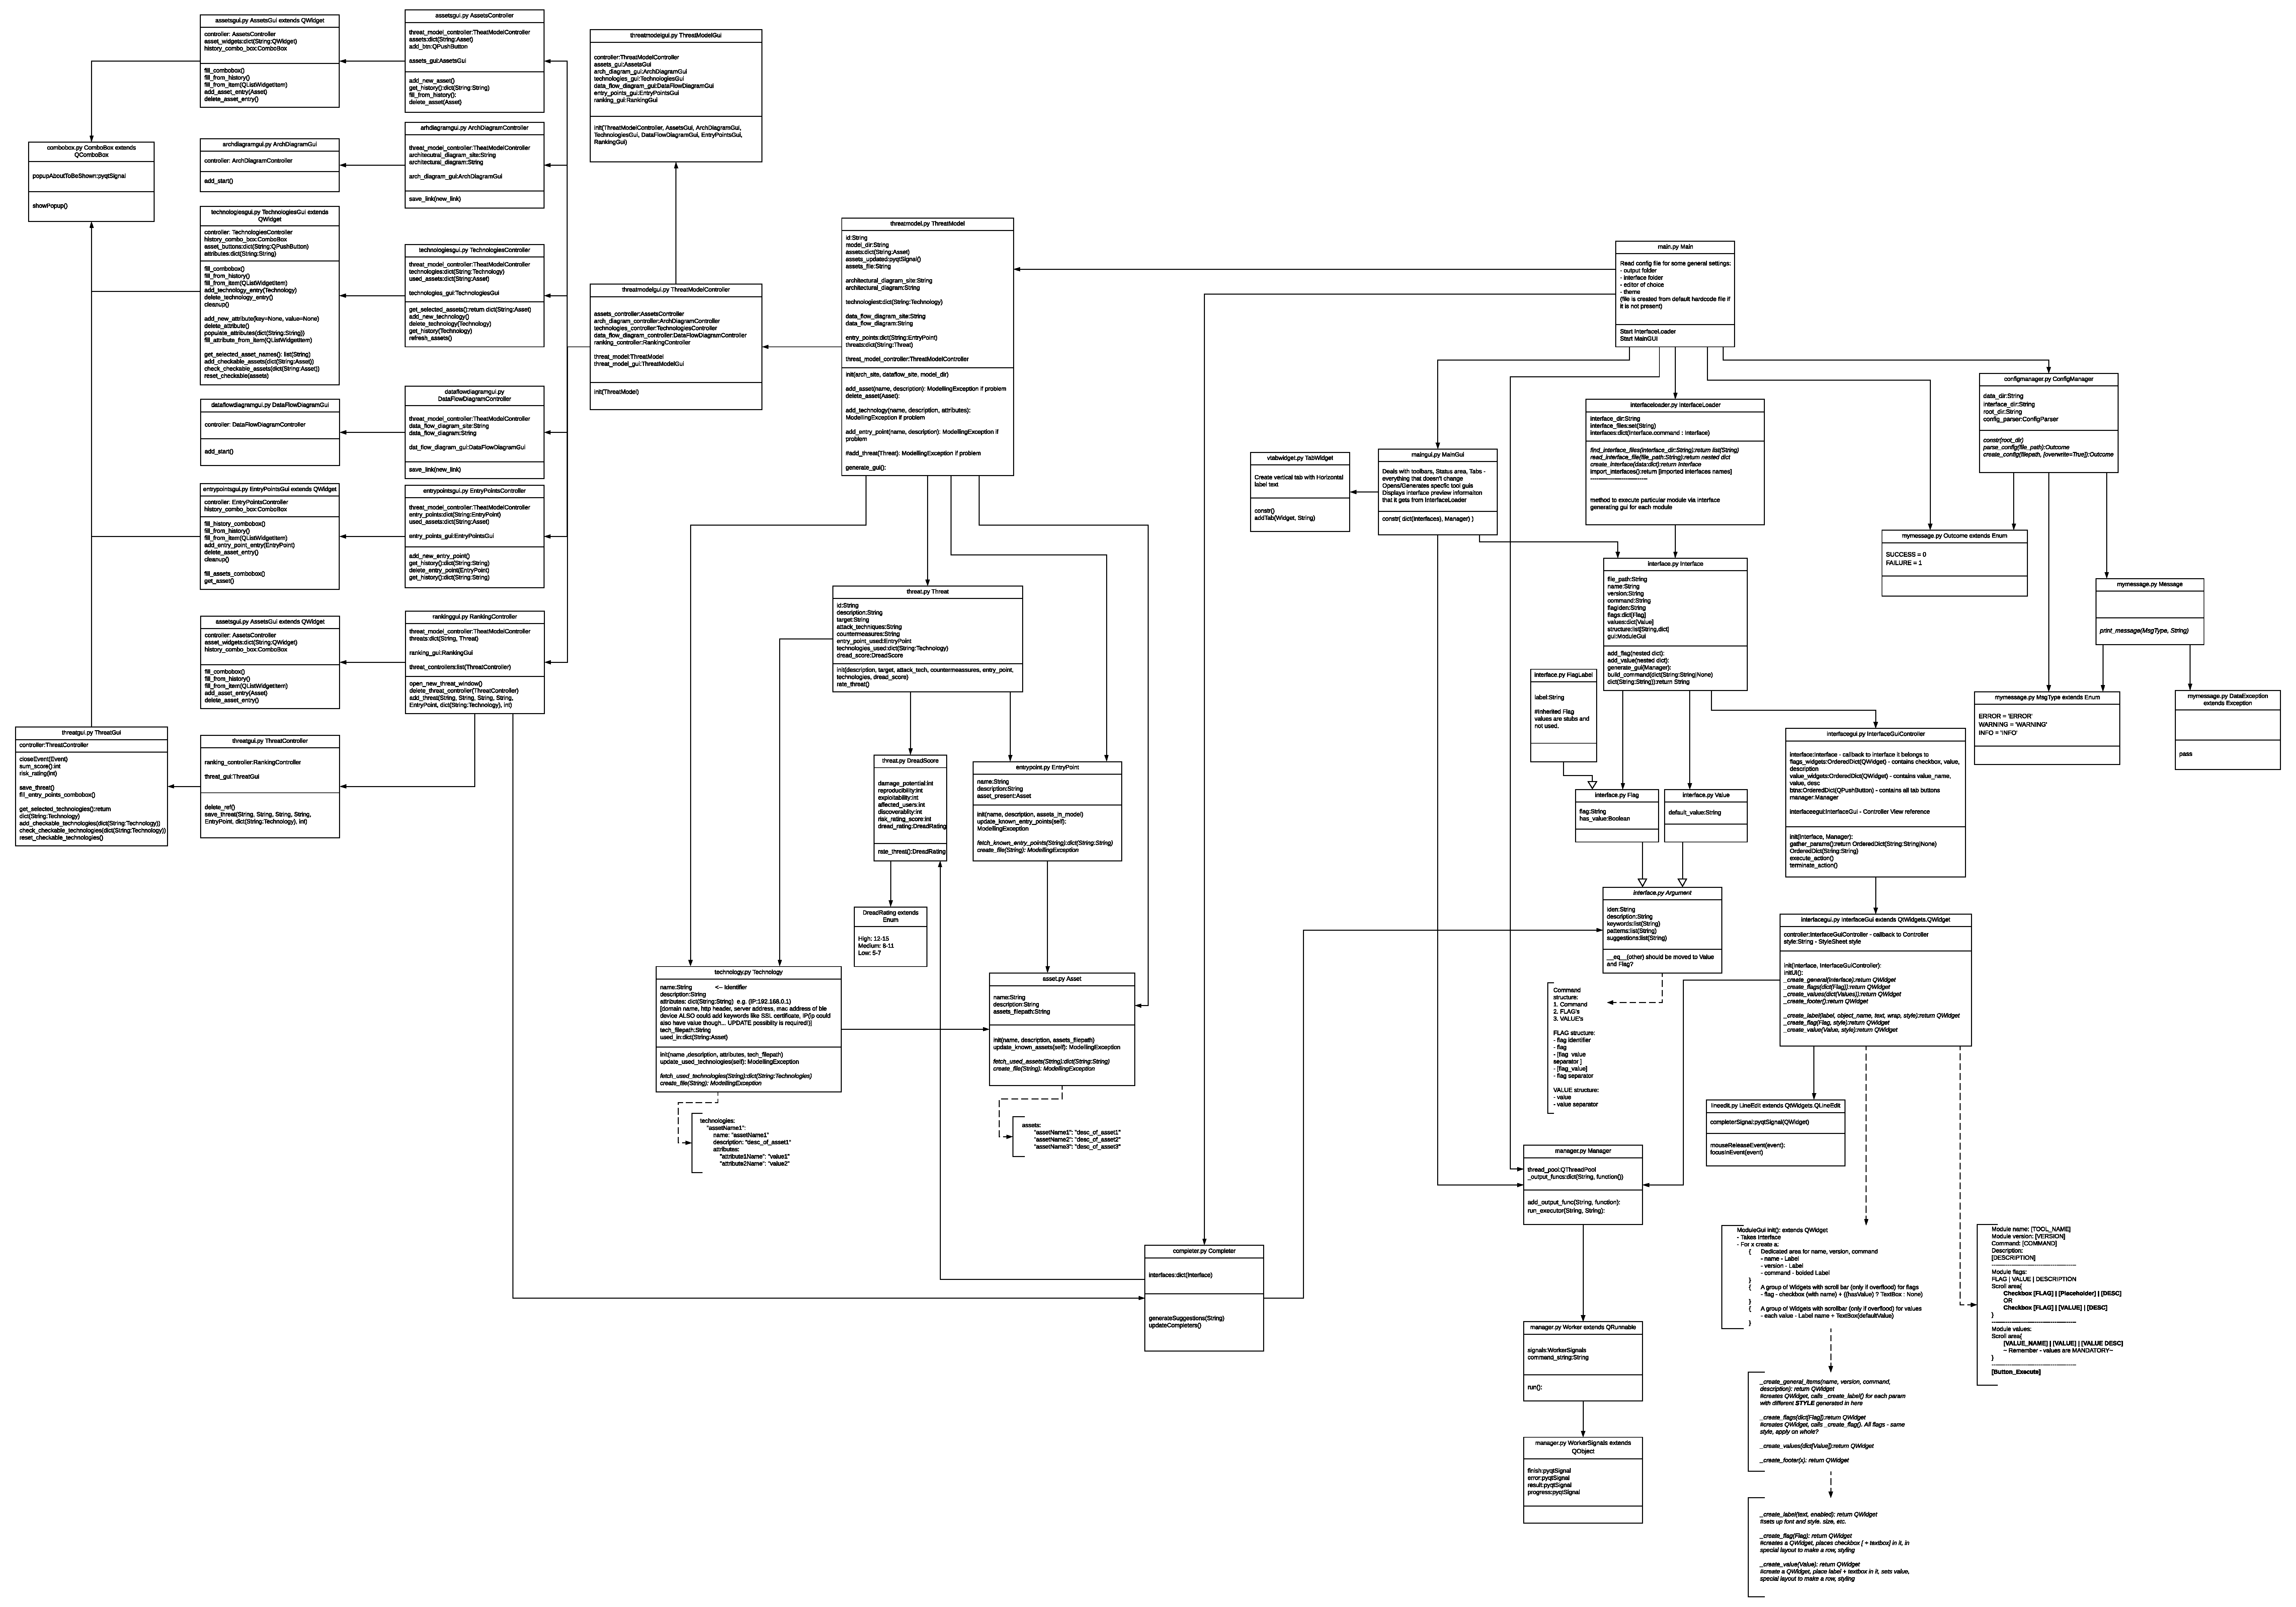
\includegraphics[width=\linewidth,keepaspectratio]{overall_class_diagram}
			\captionof{figure}{Complete class diagram}
			\label{fig:xx}
		\end{minipage}
	\end{sideways}
\end{center}


\section{Project structure}\label{sec:appendix-proj-struct}

\begin{center}
	\begin{sideways}%[htbp]
		\begin{minipage}{0.92\textheight}
			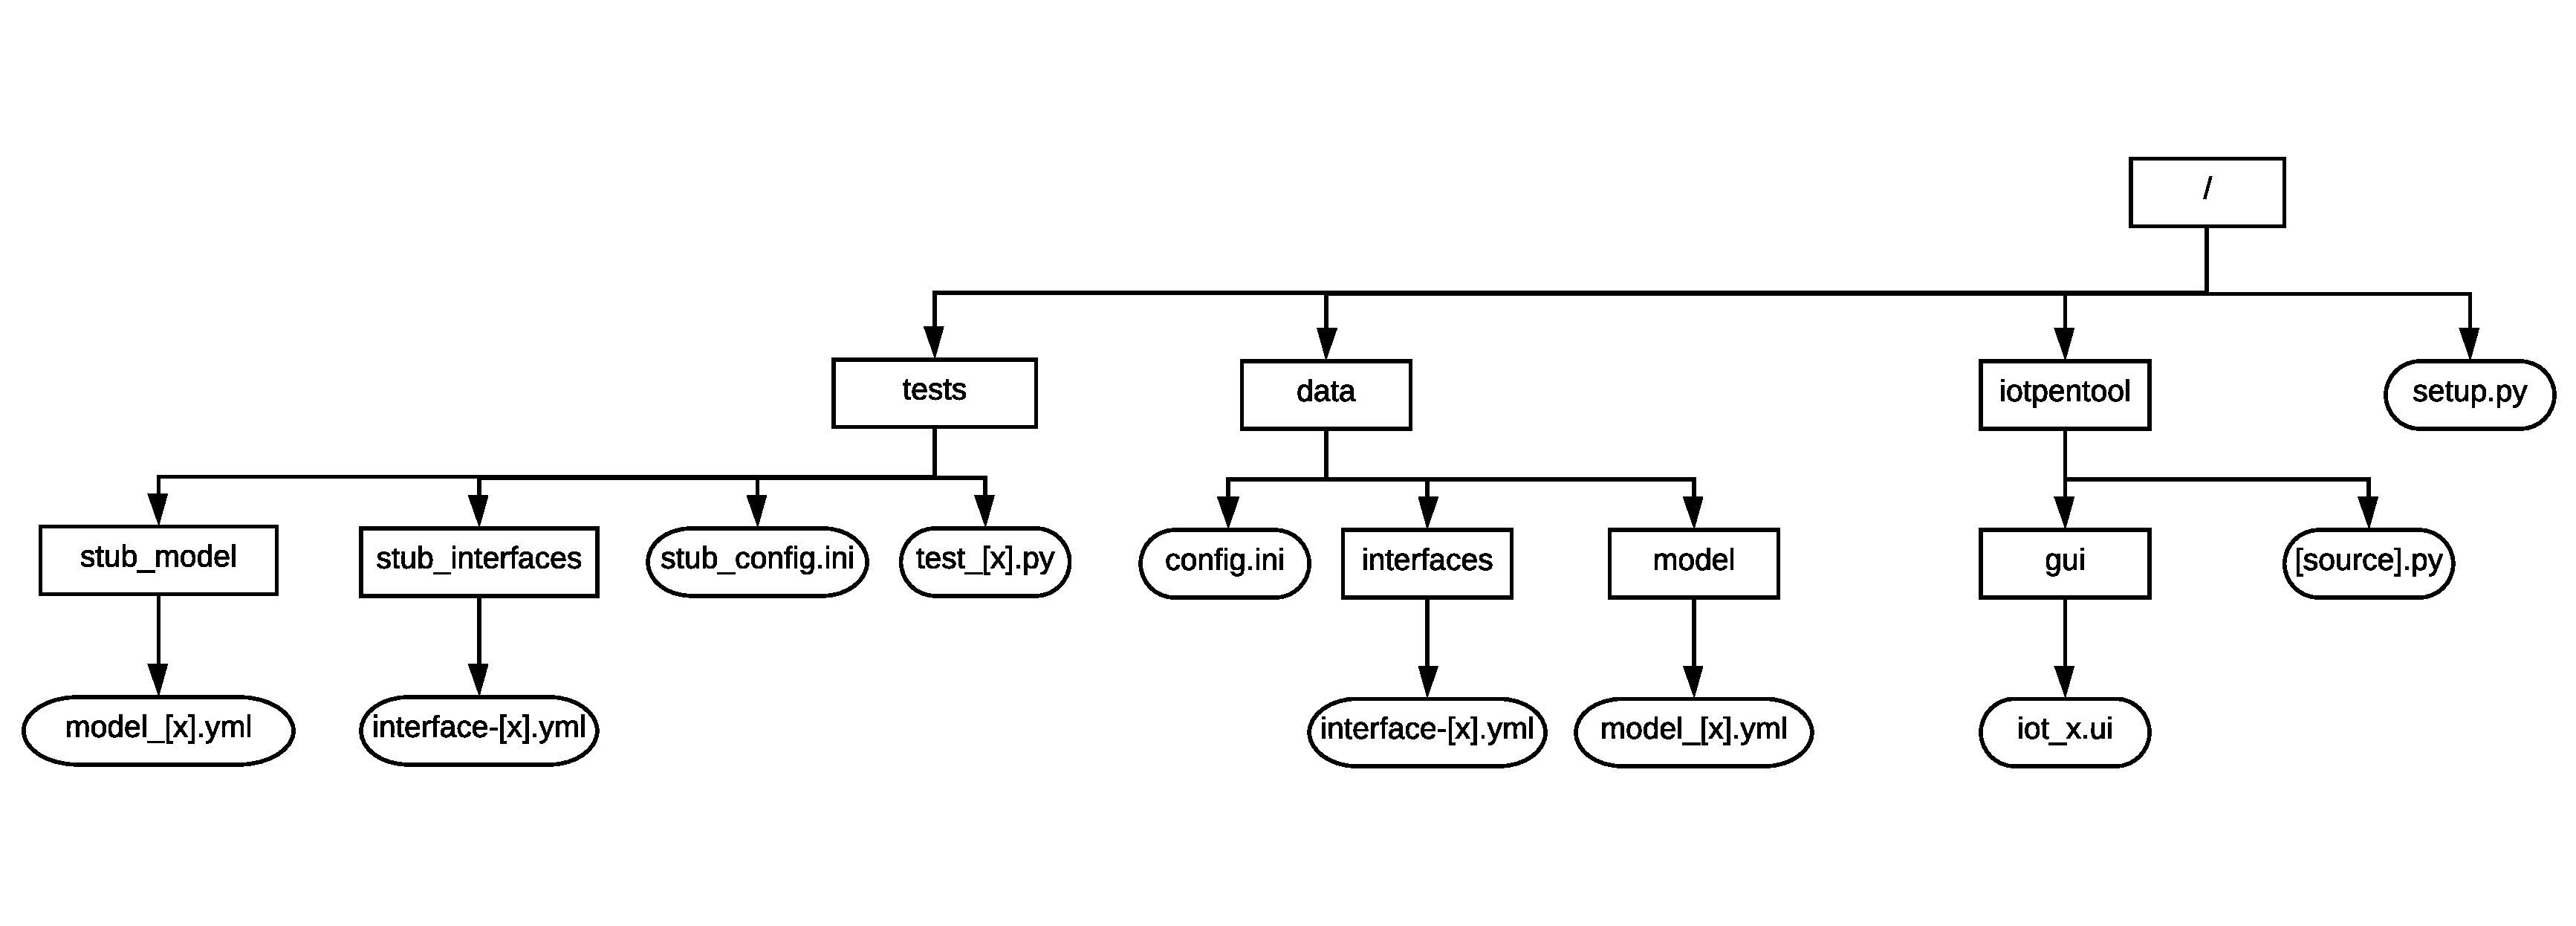
\includegraphics[width=\linewidth,keepaspectratio]{project_layout}
			\captionof{figure}{Project layout}
			\label{fig:xx}
		\end{minipage}
	\end{sideways}
\end{center}


\section{Interface file structure} \label{sec:appendix-interface-struct}
\begin{figure}[!htb]
	\center{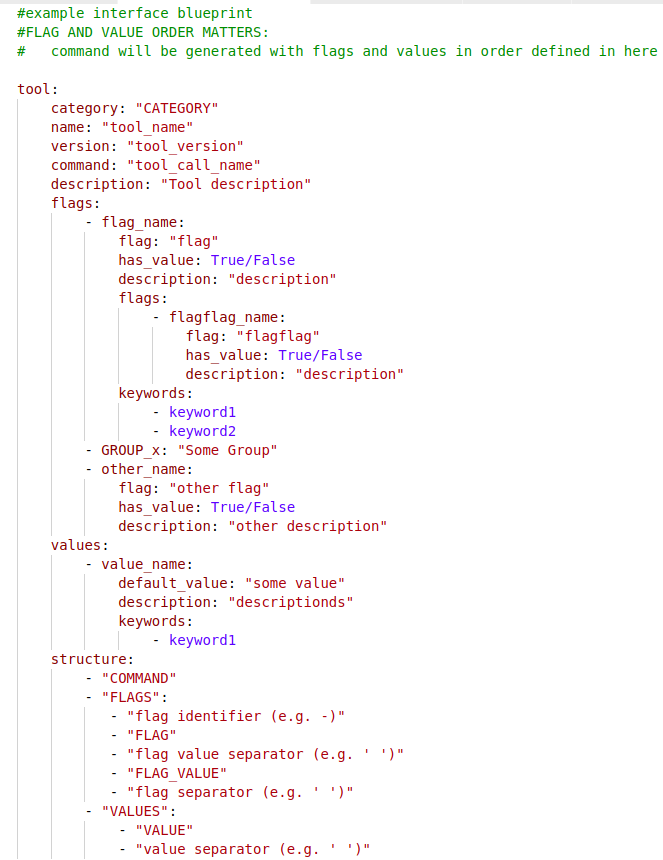
\includegraphics[width=\textwidth]
		{config_struct.png}}
	\caption{\label{fig:interface-struct1} Interface file structure}
\end{figure}


\section{Software tests table}\label{sec:appendix-software-tests}

\begin{figure}[!htb]
	\center{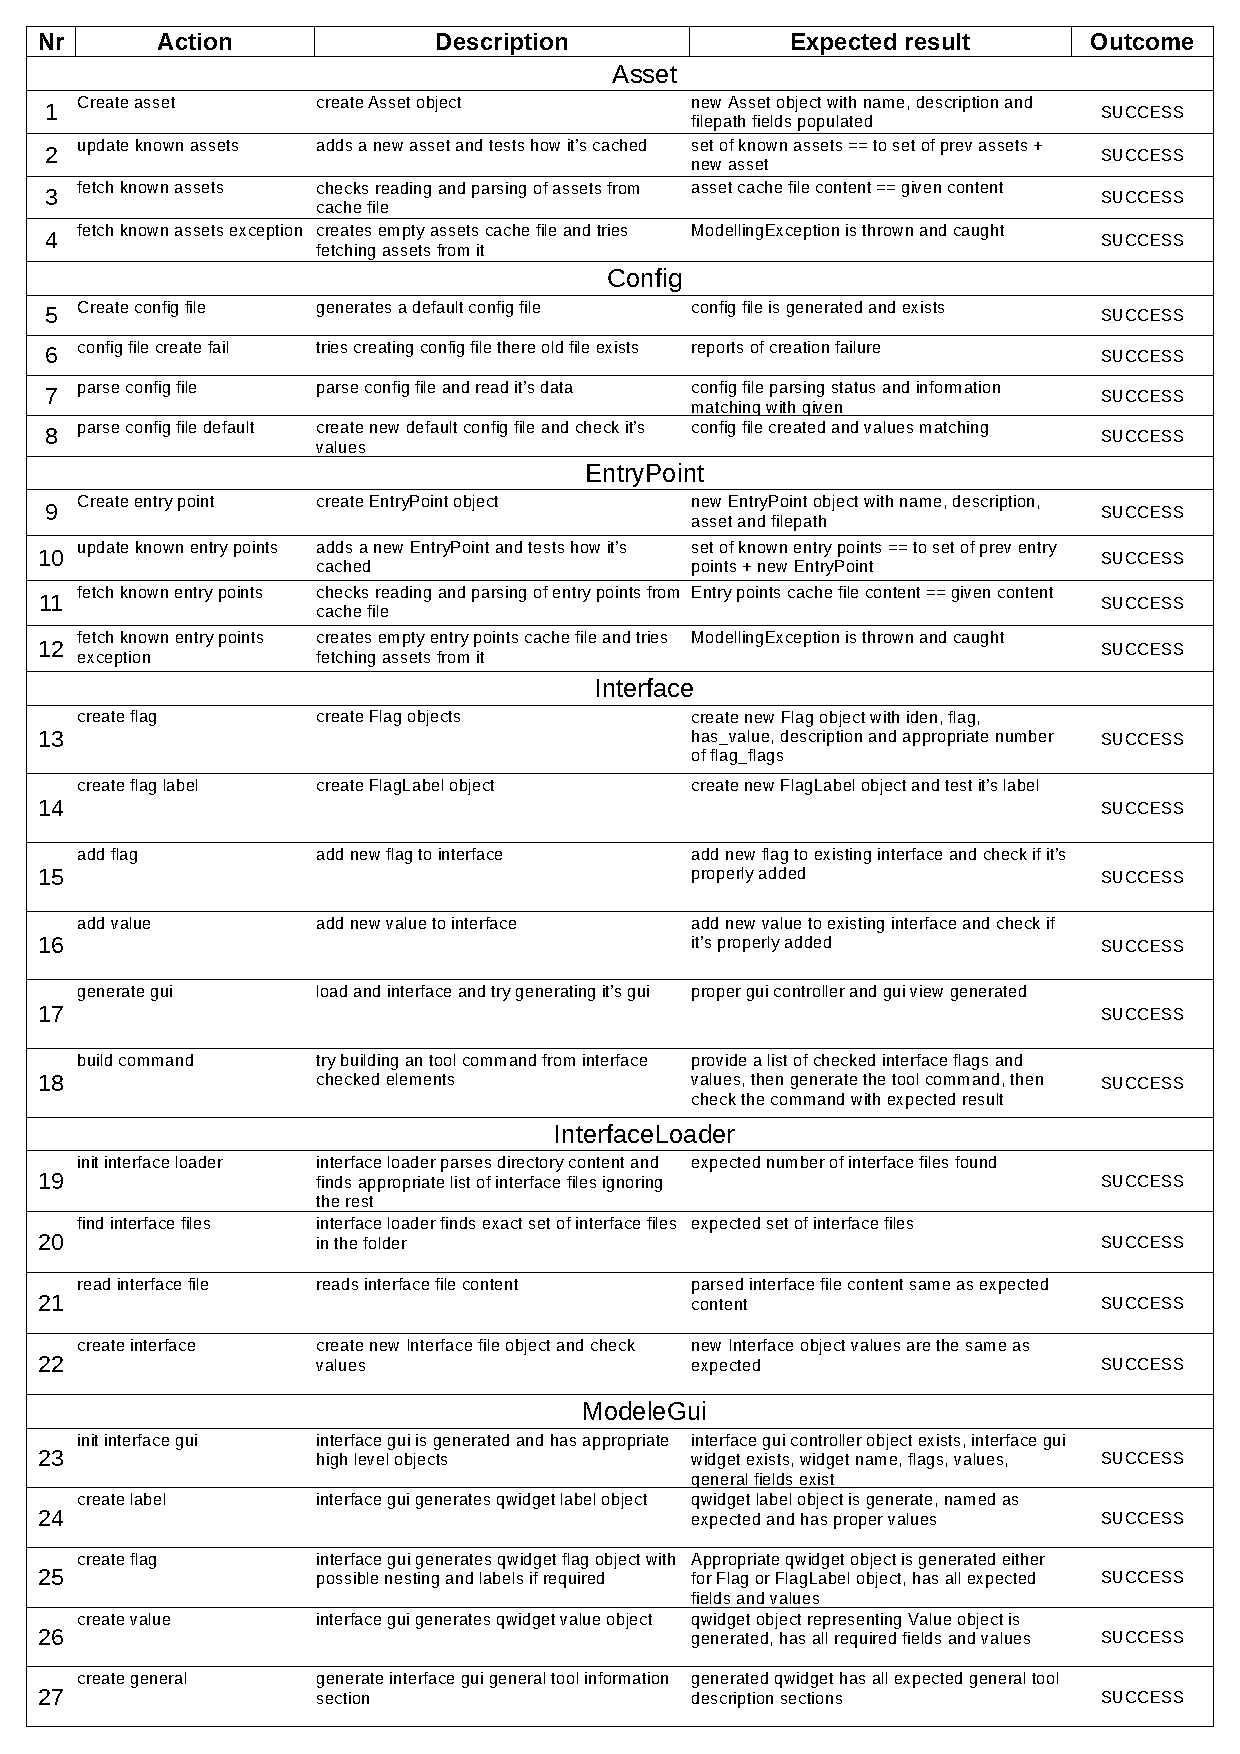
\includegraphics[width=\textwidth]
		{test_table1.pdf}}
	\caption{Test table part 1}
\end{figure}

\begin{figure}[!htb]
	\center{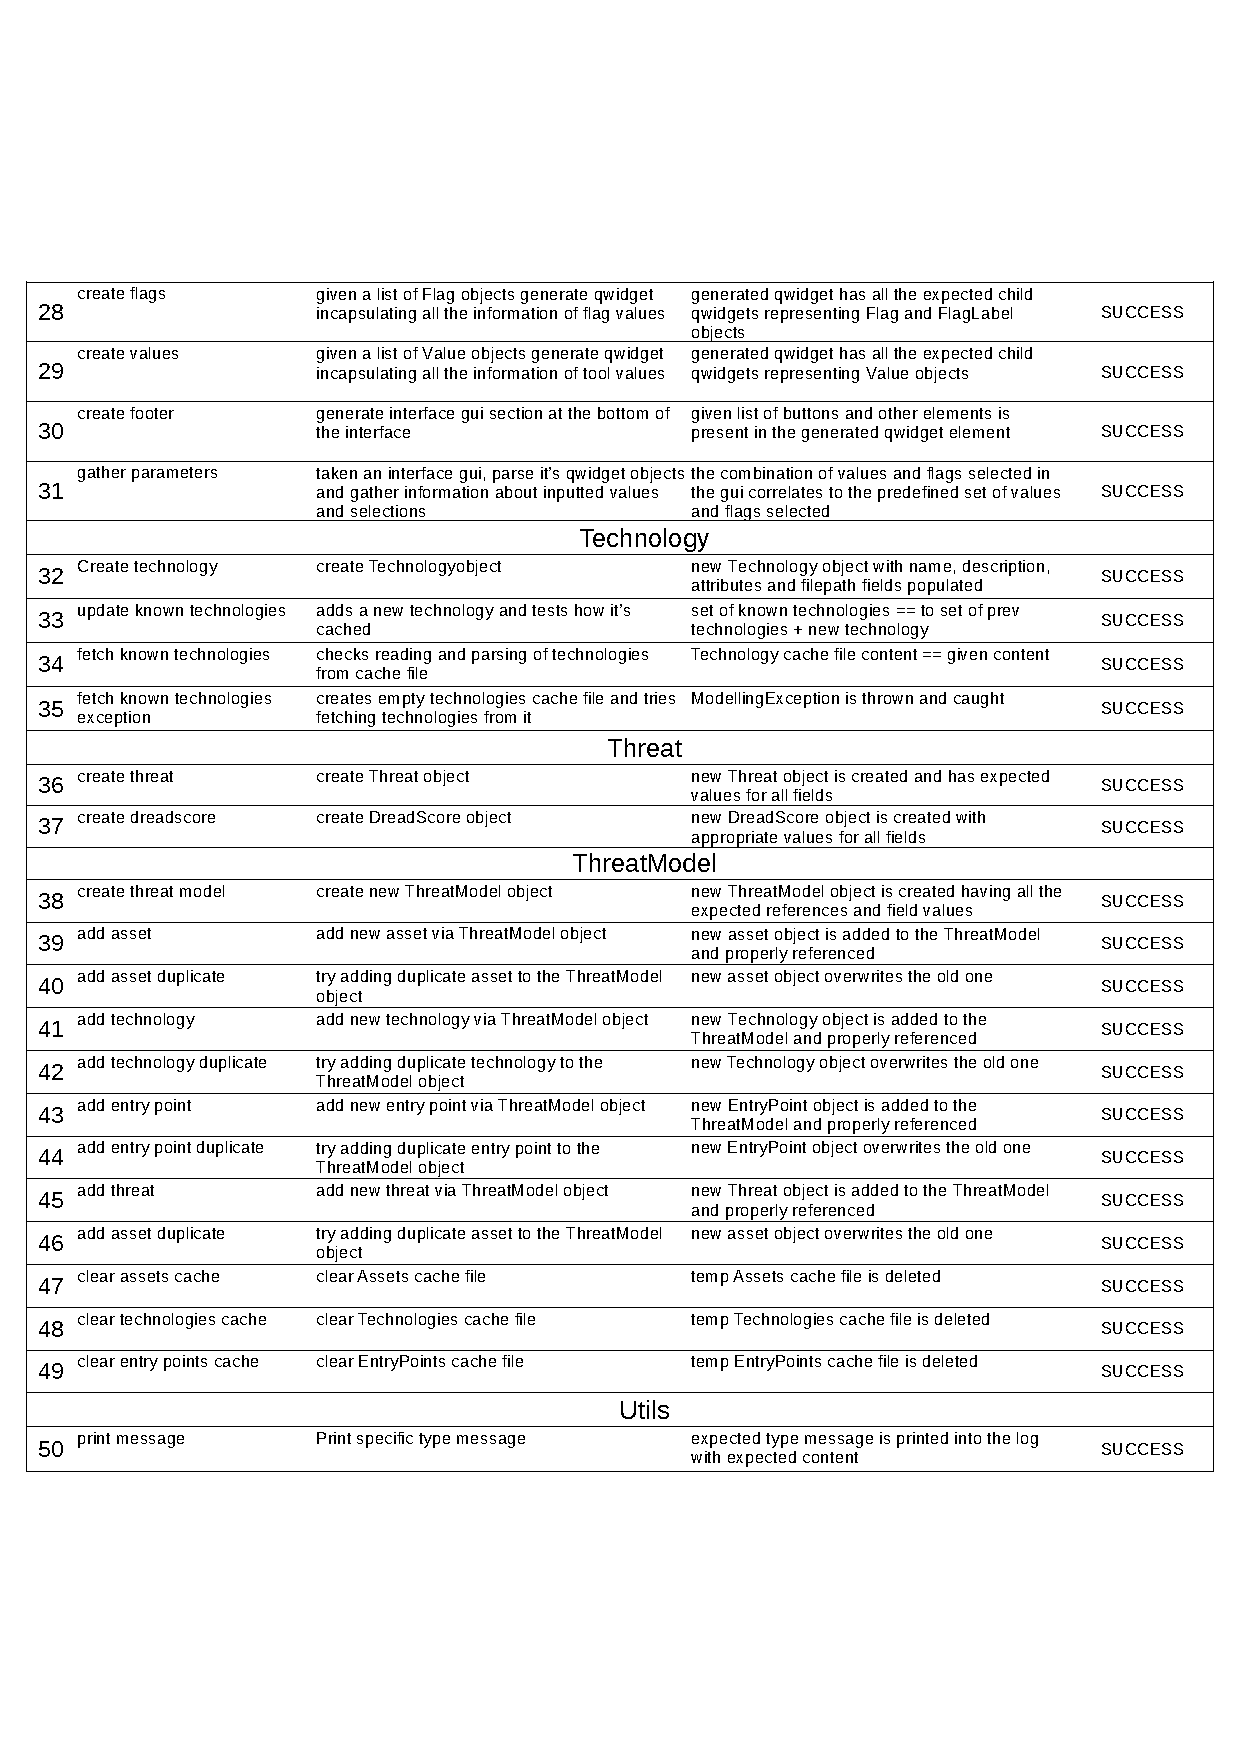
\includegraphics[width=\textwidth]
		{test_table2.pdf}}
	\caption{ Test table part 2}
\end{figure}


\section{Sprint plans}\label{sec:appendix-sprint-plans}
\begin{center}
	\begin{sideways}%[htbp]
		\begin{minipage}{0.92\textheight}
			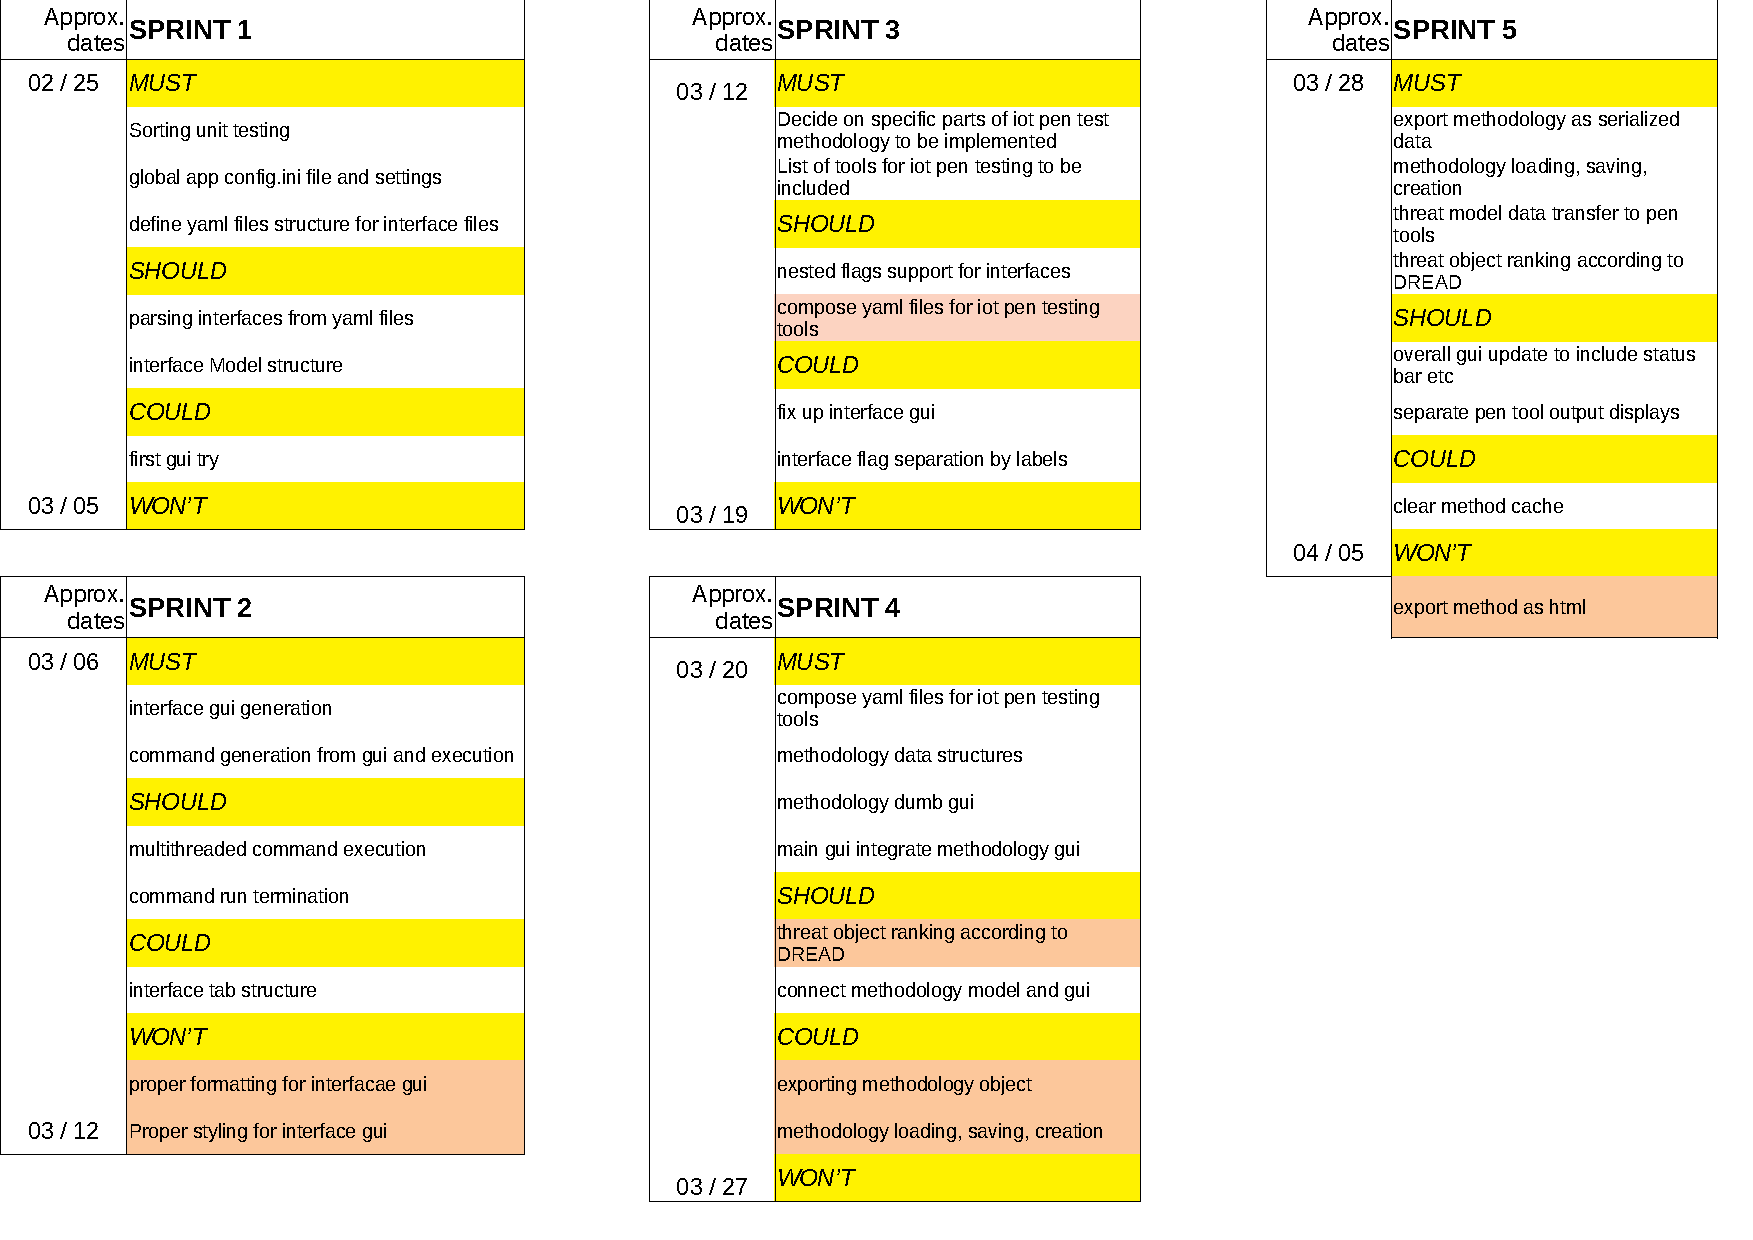
\includegraphics[width=\linewidth,keepaspectratio]
			{sprint_planning.pdf}
			\captionof{figure}{Sprint plans}
			\label{fig:xx}
		\end{minipage}
	\end{sideways}
\end{center}


\section{Github statistics}\label{sec:appendix-github}
\begin{figure}[!htb]
	\center{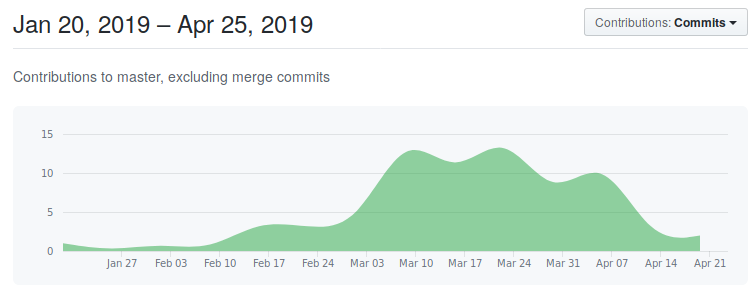
\includegraphics[width=\textwidth]
		{commit-graph.png}}
	\caption{Project commit history}
\end{figure}

\begin{figure}[!htb]
	\center{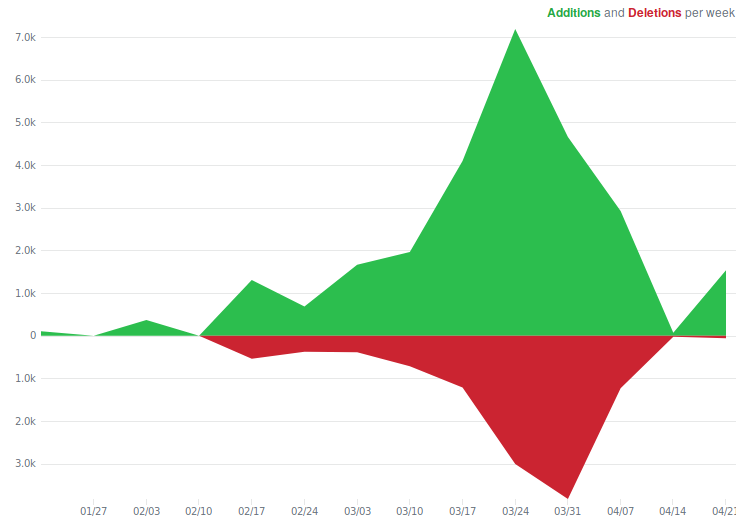
\includegraphics[width=\textwidth]
		{code-graph.png}}
	\caption{Code frequency}
\end{figure}


\section{Gannt charts}\label{sec:appendix-gantt}
\begin{center}
	\begin{sideways}%[htbp]
		\begin{minipage}{0.92\textheight}
			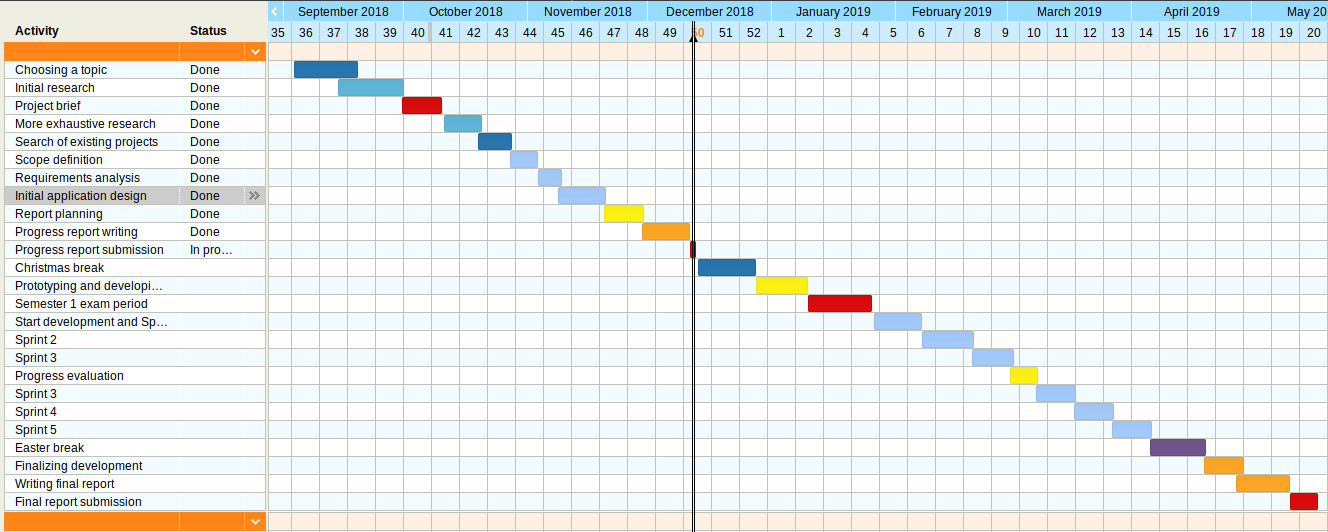
\includegraphics[width=\linewidth,keepaspectratio]
			{Gannt.png}
			\captionof{figure}{Expected project schedule}
			\label{fig:xx}
		\end{minipage}
	\end{sideways}
\end{center}

\begin{center}
	\begin{sideways}%[htbp]
		\begin{minipage}{0.92\textheight}
			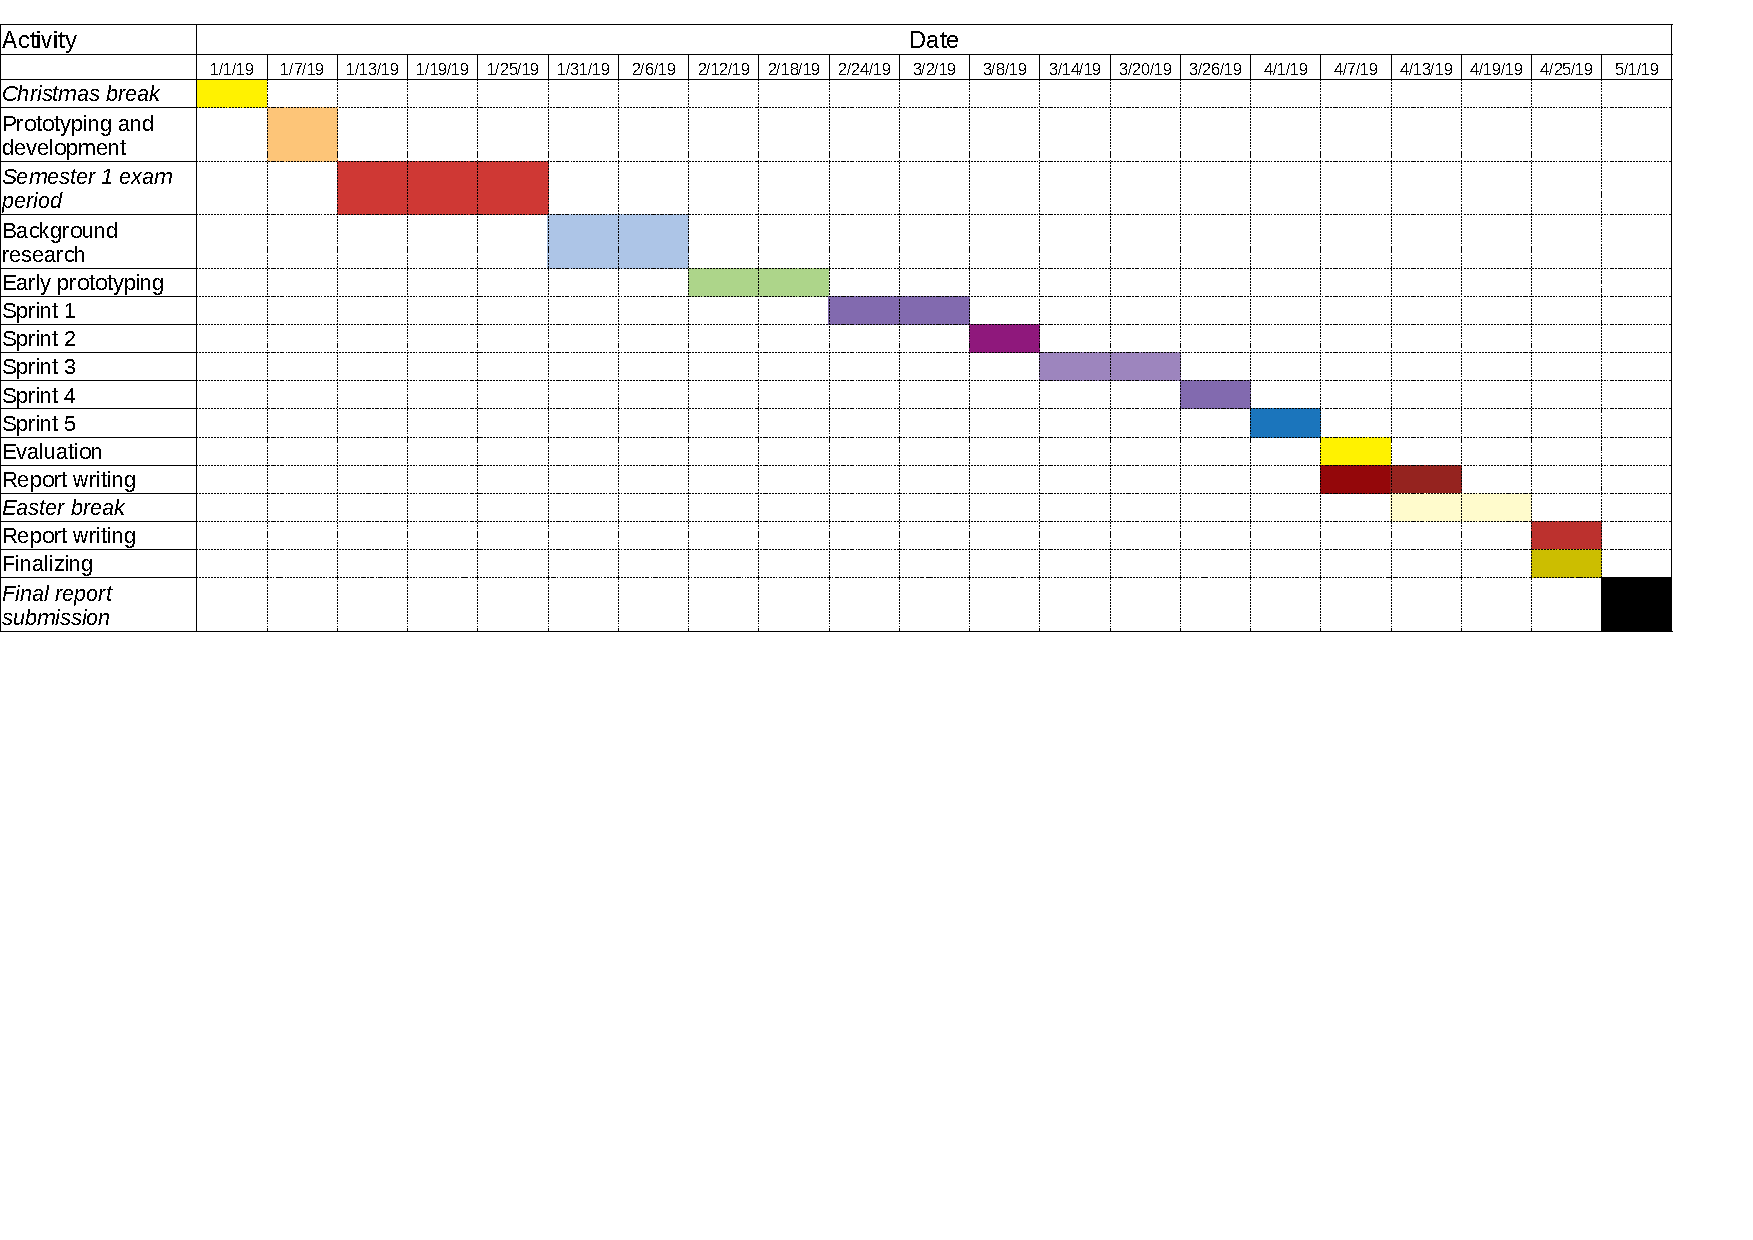
\includegraphics[width=\linewidth,keepaspectratio]
			{final-gannt.pdf}
			\captionof{figure}{Actual project schedule for Semester 2}
			\label{fig:xx}
		\end{minipage}
	\end{sideways}
\end{center}


\section{Risk management} \label{sec:appendix-risk}
Probability and Impact are rated in a scale from 1 to 5.

\def\riska{Loss of source code at some stage of development}
\def \probabilitya {1}
\def \impacta {4}
\def \mitigationa {Use of remote source control  repository to frequently record every stage of the development, thus being able to recover it if needed. }

\def\riskaa{Unable to fulfill all of the requirements due to technical implemention difficulties}
\def \probabilityaa {3}
\def \impactaa {2}
\def \mitigationaa {At the start of development process requirements will be split into tasks, divided into sprints and ranked using MoSCoW prioritization, therefore ensuring that core functionality will be implemented first and a working proof of concept is available at the end of the project }

\def\riskaaa{Insufficient time to develop a prototype due to other course modules}
\def \probabilityaaa {2}
\def \impactaaa {2}
\def \mitigationaaa {Dedicate fixed amount of time every week for the project in order to keep up with the schedule }

\def\riskaaaa{Some part of the project taking up significantly longer that expected}
\def \probabilityaaaa {3}
\def \impactaaaa {2}
\def \mitigationaaaa {Re-evaluate task importance and re-adjust development schedule in order to deliver functional product }

\def\riskaaaaa{Unable to complete adequate application testing due to technical or time limitations}
\def \probabilityaaaaa {3}
\def \impactaaaaa {3}
\def \mitigationaaaaa {Complete limited or partial testing concentrating on core functionality, document causes and reasoning. If difficulties arise in early stages of development  due to technical limitations, seek support from university staff that are experienced in such situations. }

\def\riskaaaaaa{Development is halted as additional research is needed}
\def \probabilityaaaaaa {3}
\def \impactaaaaaaa {2}
\def \mitigationaaaaaa {Re-adjust project schedule and shorten over planned activities in order to accompany expected delay.}


\def\riskaaaaaaa{it is impossible to achieve a requirement during the given time frame}
\def \probabilityaaaaaaa {1}
\def \impactaaaaaa {2}
\def \mitigationaaaaaaa {Alter project goals to be more realistic and update time schedule taking that into account. Impact largely depends on the stage of development. In the prototyping period impact is insignificant, although, in later stages can become troublesome}


\begin{center}
	\begin{tabular}{ |m{5cm}|m{2cm}|m{1cm}|m{6cm}| } 
		\hline
		Risk & Probably & Impact & Mitigation \\ 
		\hline
		\riska & \probabilitya & \impacta & \mitigationa \\ 
		\hline
		\riskaa & \probabilityaa & \impactaa & \mitigationaa \\ 
		\hline
		\riskaaa & \probabilityaaa & \impactaaa & \mitigationaaa \\ 
		\hline
		\riskaaaa & \probabilityaaaa & \impactaaaa & \mitigationaaaa \\ 
		\hline
		\riskaaaaa & \probabilityaaaaa & \impactaaaaa & \mitigationaaaaa \\ 
		\hline
		\riskaaaaaa & \probabilityaaaaaa & \impactaaaaaa & \mitigationaaaaaa \\ 
		\hline
		\riskaaaaaaa & \probabilityaaaaaaa & \impactaaaaaaa & \mitigationaaaaaaa \\ 
		\hline
	\end{tabular}
\end{center}

\section{Content of Design Archive}
\begin{itemize}
	\item \textbf{'data' folder} containing 10 interface .yml files, some generated cache files, \textbf{config.ini} file
	\item \textbf{'iotpentool' folder} containing the whole source code
	\item \textbf{'tests' folder} containing all the test data and files
	\item alert\_system.pickle file saved Alert system threat model file
	\item \textbf{'diagram\_icon.png' file} icon used and taken from (https://pixabay.com/illustrations/diagram-icon-business-symbol-chart-2008478/)
	\item \textbf{'export.json' file} exported Alert system threat model data
	\item \textbf{'unit\_inte\_test\_report.html' file} Unit - Integration test auto-generated report.
	\item \textbf{'media' folder} containing all the graphs and diagrams used in the report.
\end{itemize}


\section{Pentesting screenshots}\label{sec:appendix-pen-testing}

\begin{figure}[!htb]
	\center{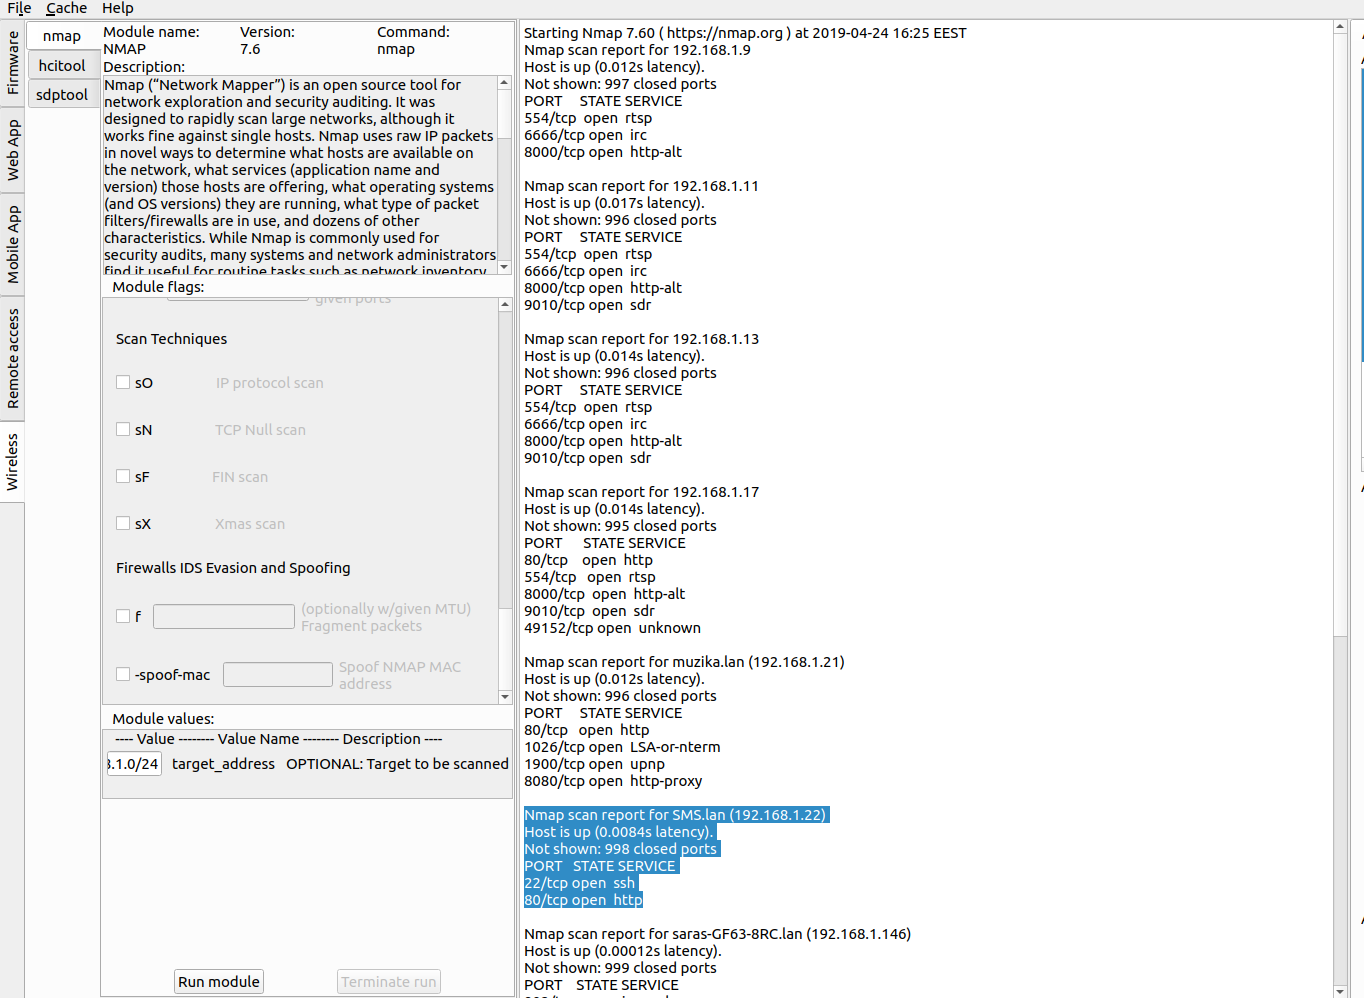
\includegraphics[width=\textwidth]
		{screenshots/nmap_network.png}}
	\caption{Nmap network scan}
\end{figure}

\begin{figure}[!htb]
	\center{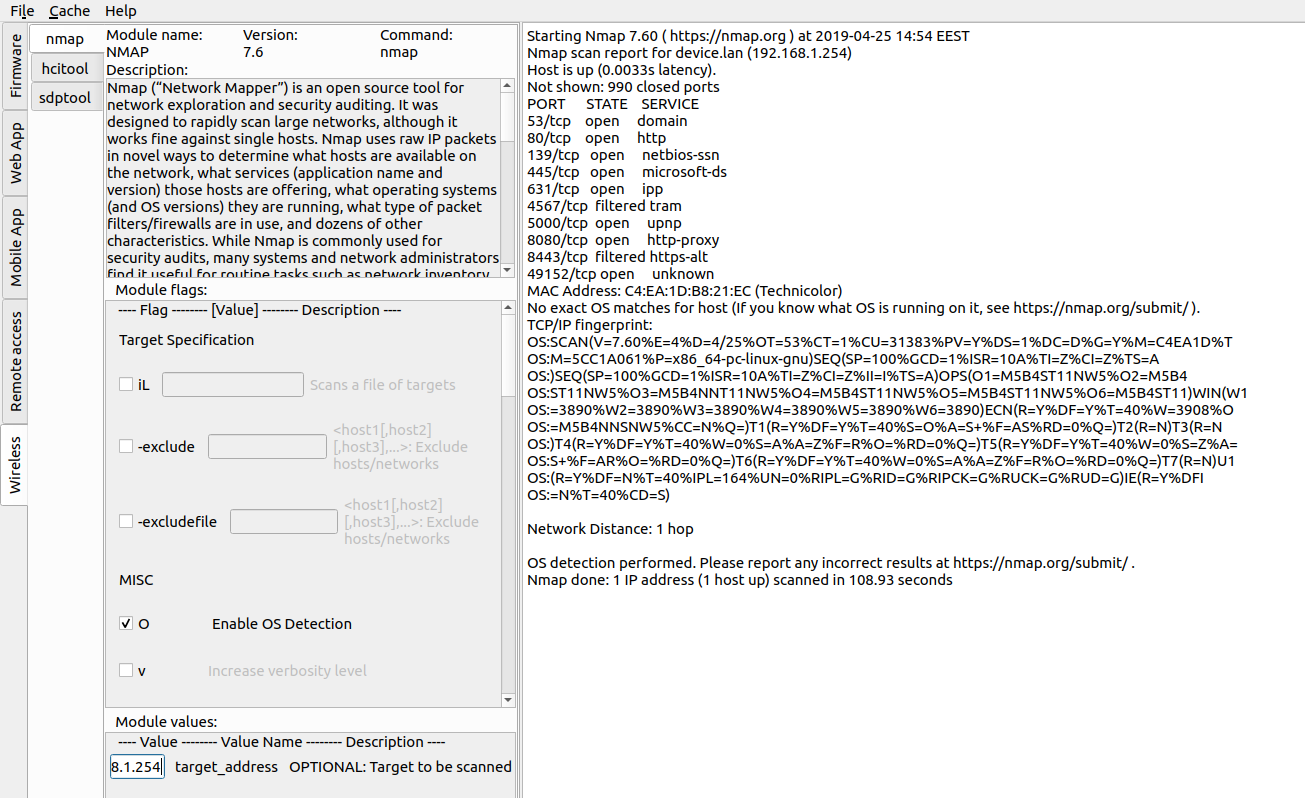
\includegraphics[width=\textwidth]
		{screenshots/nmap_router.png}}
	\caption{Nmap router port scan}
\end{figure}

\begin{figure}[!htb]
	\center{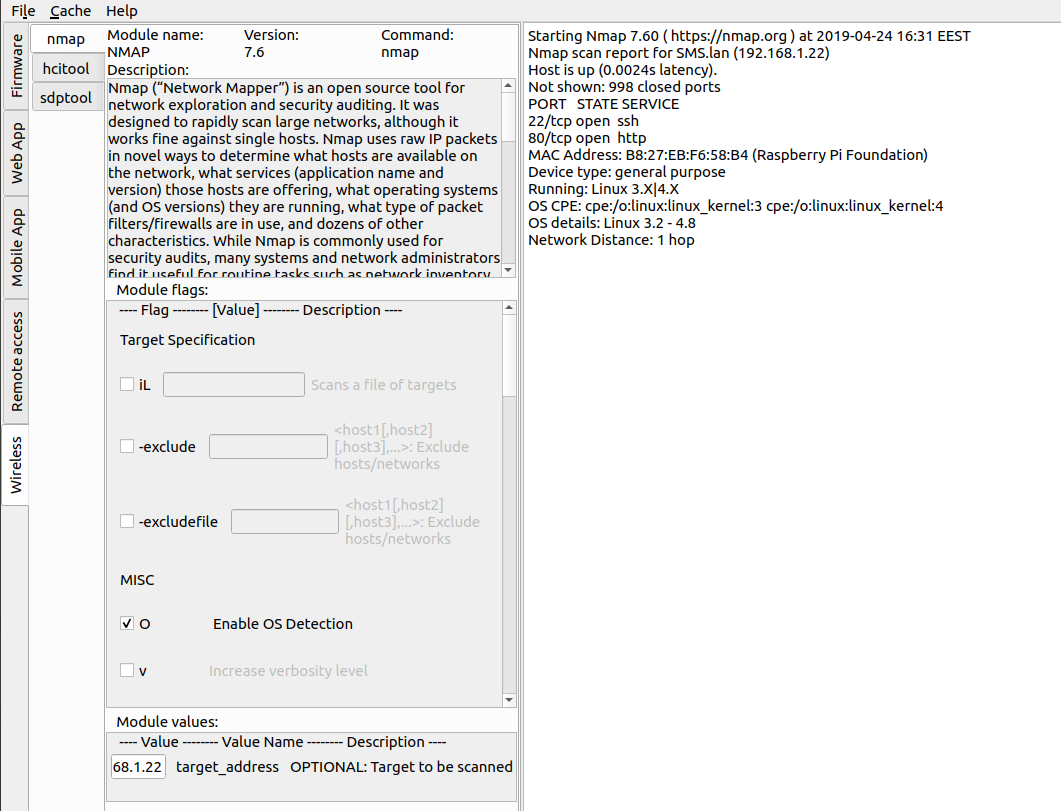
\includegraphics[width=\textwidth]
		{screenshots/nmap_port.png}}
	\caption{Nmap system hub port scan}
\end{figure}

\begin{figure}[!htb]
	\center{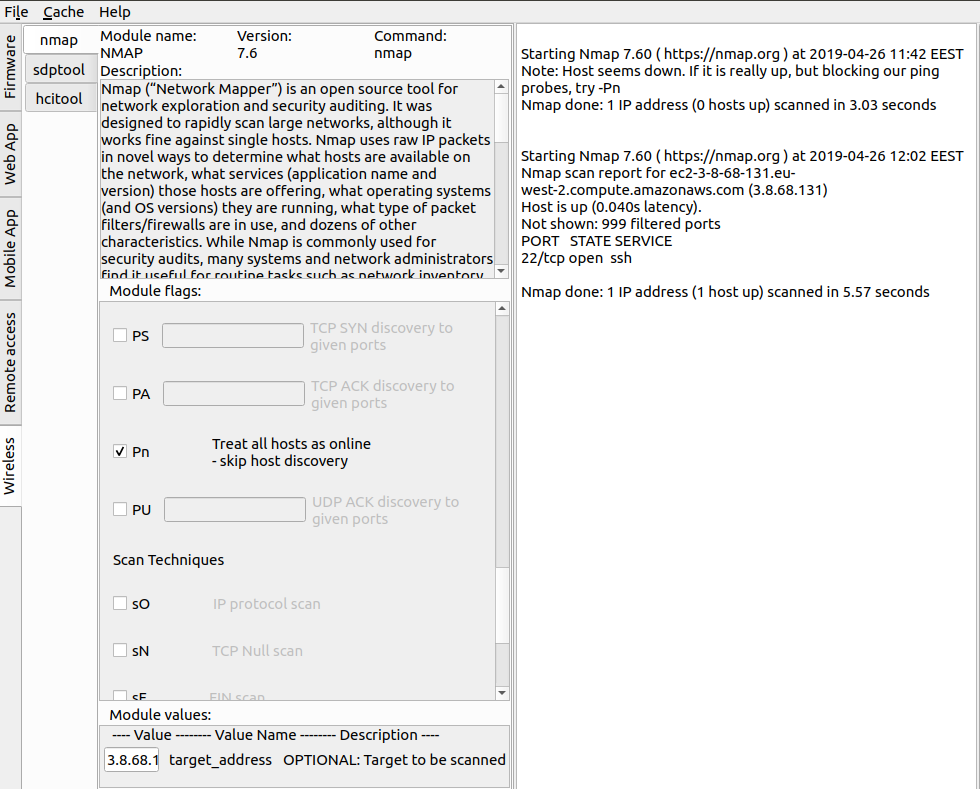
\includegraphics[width=\textwidth]
		{screenshots/nmap_cloud.png}}
	\caption{Nmap cloud server port scan}
\end{figure}

\begin{figure}[!htb]
	\center{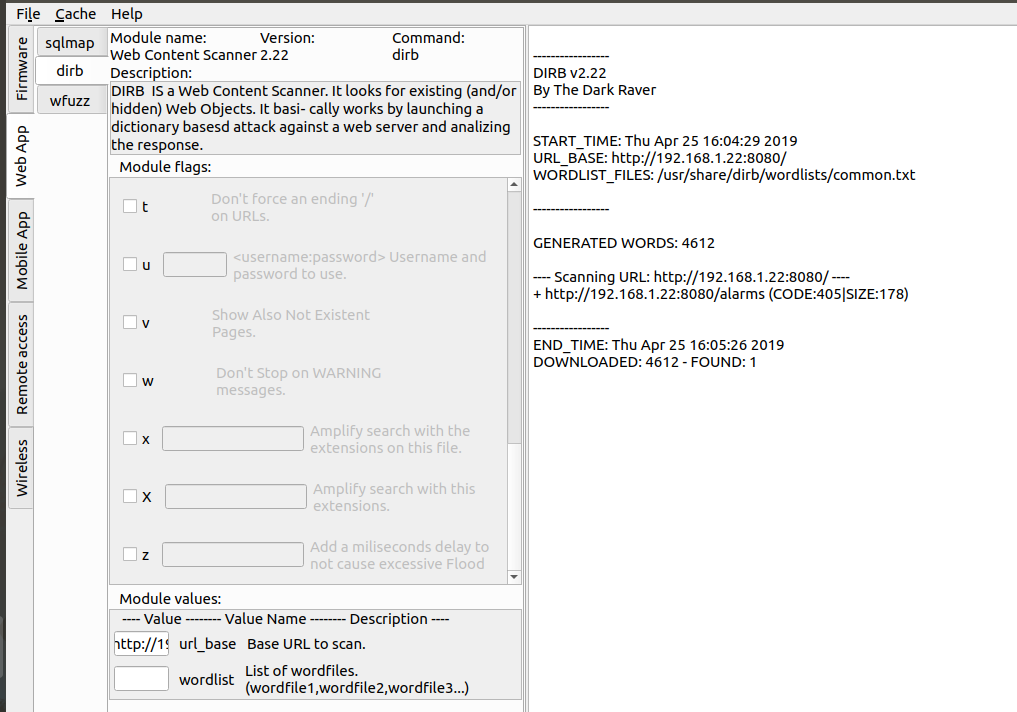
\includegraphics[width=\textwidth]
		{screenshots/dirb.png}}
	\caption{Dirb system hub API fuzzing}
\end{figure}

\begin{figure}[!htb]
	\center{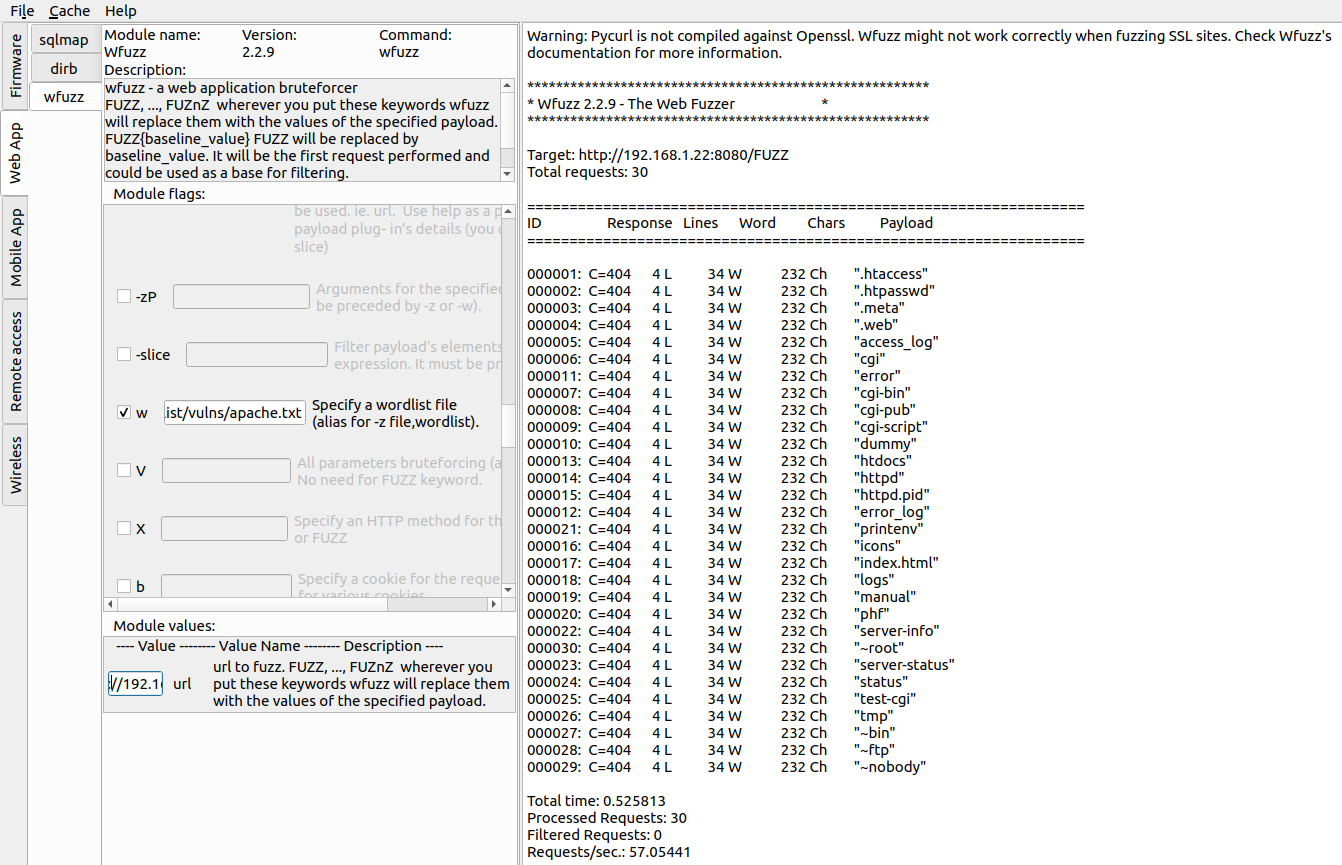
\includegraphics[width=\textwidth]
		{screenshots/wfuzz_run.png}}
	\caption{Wfuzz running against system hub API}
\end{figure}

\begin{figure}[!htb]
\center{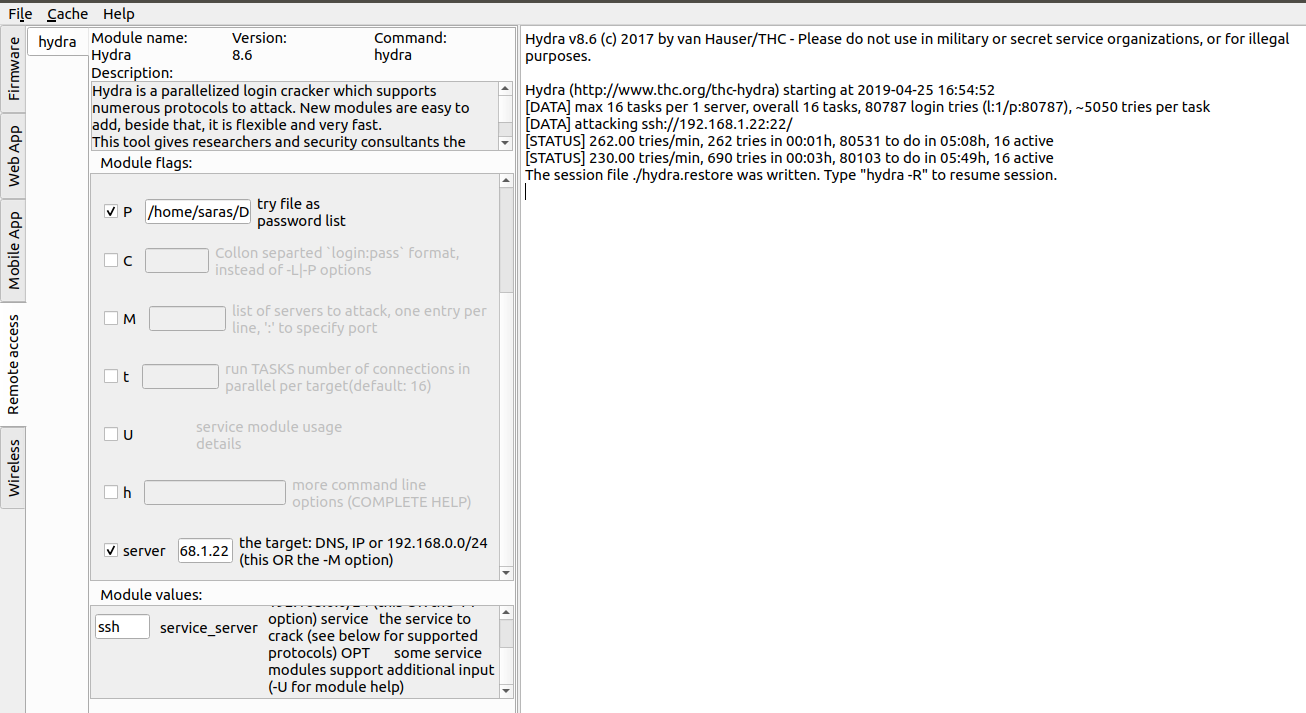
\includegraphics[width=\textwidth]
	{screenshots/hydra_run.png}}
\caption{Brute forcing system hub SSH password}
\end{figure}

\begin{figure}[!htb]
\center{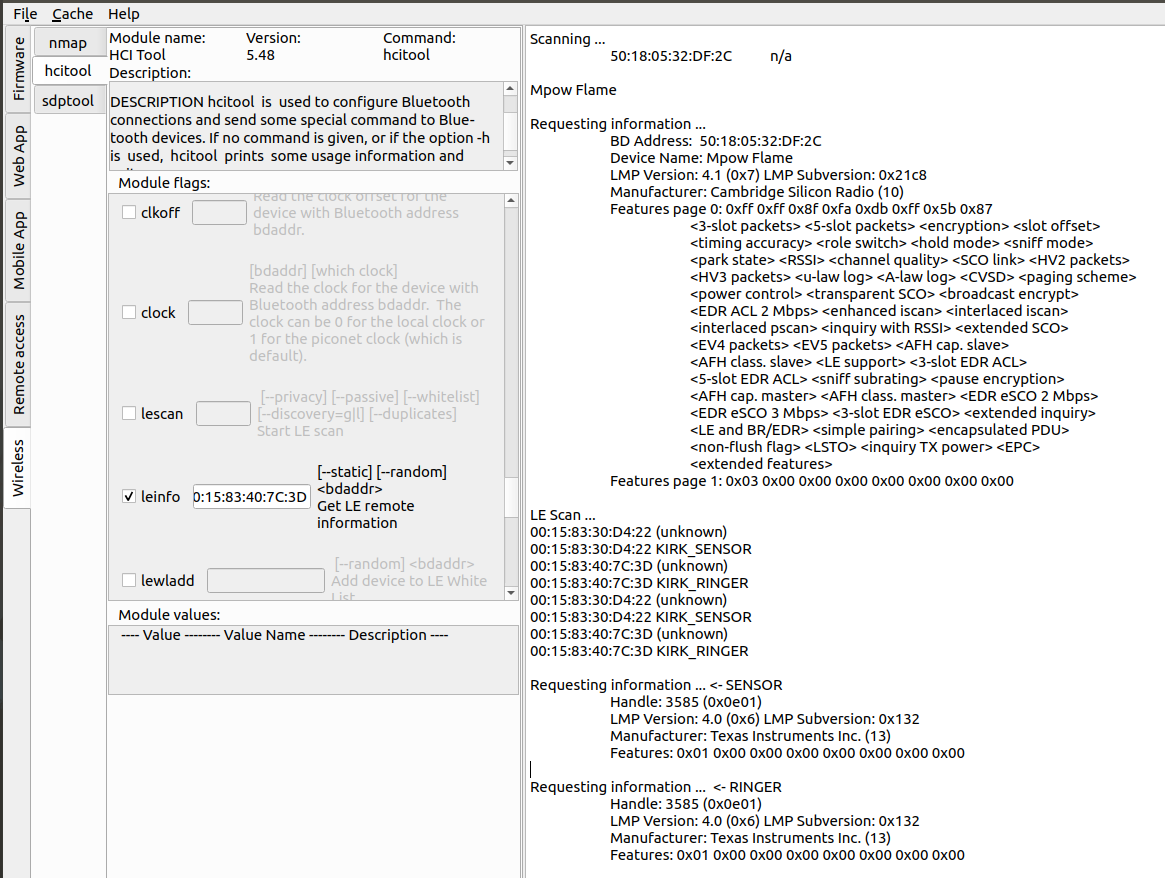
\includegraphics[width=\textwidth]
	{screenshots/hcitool_scan.png}}
\caption{Hcitool BLE device scan}
\end{figure}

\begin{figure}[!htb]
\center{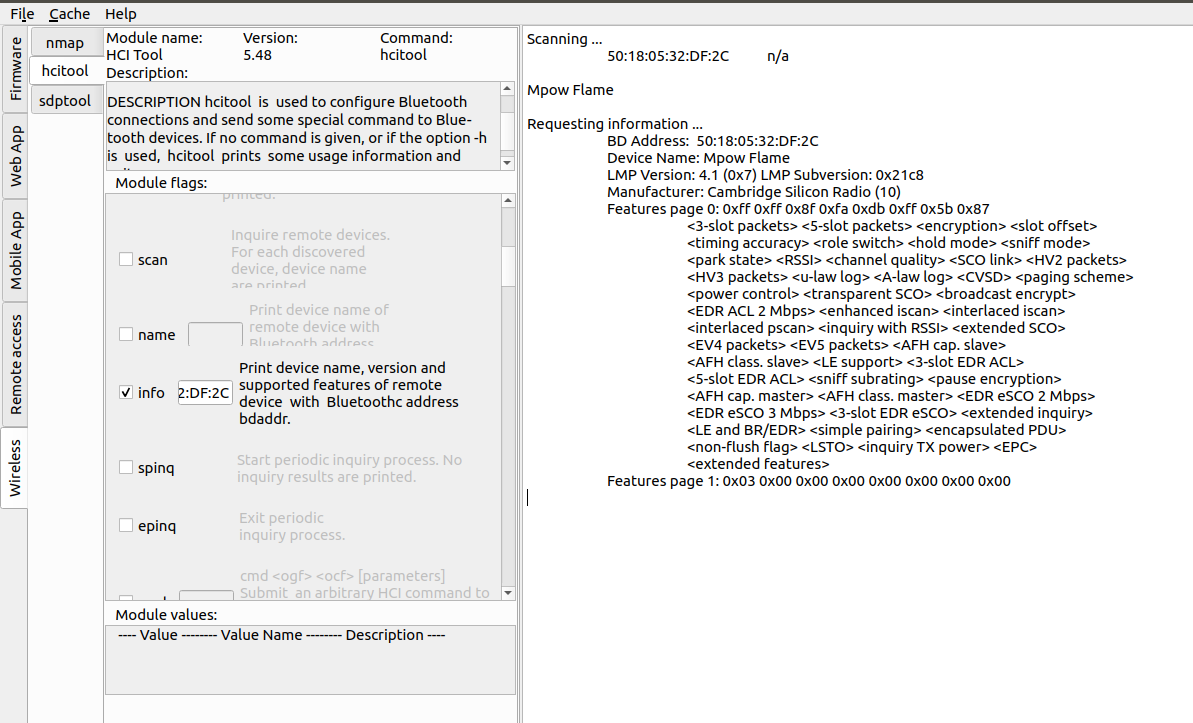
\includegraphics[width=\textwidth]
	{screenshots/hcitool_info.png}}
\caption{Hcitool displaying BLE device information}
\end{figure}


\end{document}
